\documentclass[11pt]{article}
\usepackage[review]{acl}
\usepackage{times}
\usepackage{latexsym}
\usepackage[T1]{fontenc}
\usepackage[utf8]{inputenc}
\usepackage{microtype}
\usepackage{graphicx}
\usepackage{booktabs}
\usepackage{amsmath}
\usepackage{amssymb}
\usepackage{multirow}

\newcommand{\ds}{DeepSeek}
\newcommand{\qw}{Qwen}
\newcommand{\mm}{MiniMax}
\newcommand{\ci}[2]{$[#1,\,#2]$}

\title{Reaching Versus Selecting: What Self-Critique Adds\\to a Language Model's Answer}

\author{Anonymous ACL submission}

\begin{document}
\maketitle

\begin{abstract}
A self-critique loop has a language model criticize its own answer and answer again.
Such loops are usually compared with independent sampling by final accuracy.
We separate two things a method must do with a question: \emph{reach} a correct answer, meaning that one appears among its answers, and \emph{select} it, meaning that its most frequent answer is correct.
We compare three methods at equal tokens: a critique loop, placebo loops whose feedback says nothing about the answer, and independent sampling.
The tests were fixed in advance and run on Humanity's Last Exam with two models and on the hard tasks of BIG-Bench Extra Hard, 800 questions each.
We find three things.
\emph{Tokens buy reach}: given the same tokens, the three methods reach about the same number of questions.
\emph{A loop buys selection}: the critique loop selects significantly more questions than independent sampling in all three settings, by 25 to 34 of 800.
\emph{The critique is not always needed}: on one model the critique loop selects significantly more than a placebo loop, while on the other a placebo loop that only says ``no problem found'' selects as many at under half the tokens.
On hard questions, self-critique does not help a model find the right answer. It helps the model settle on it.
\end{abstract}

\section{Introduction}

When a language model criticizes its own answer and tries again \citep{madaan2023selfrefine,shinn2023reflexion}, is the result better than simply sampling several answers and taking the most frequent one \citep{wang2023selfconsistency}?
Studies that compare the two report final accuracy, and several find that sampling wins at equal cost \citep{wang2025rethinking,mirzaei2026sample}.
Final accuracy mixes two questions: whether a correct answer appears among the answers a method produces, and whether the method ends up choosing it.
A method can be better at one and worse at the other.

\paragraph{Two outcomes.}
We measure both.
A question is \emph{reached} if a correct answer appears among the answers a method produces, which is the coverage of \citet{brown2024monkeys}.
A question is \emph{selected} if the most frequent of those answers is correct.

\paragraph{Three methods.}
The \emph{critique loop} is the method under study: the same model, acting as a critic, reads the question and the answer and writes doubts about them, and the solver answers again.
\emph{Independent sampling} is the usual alternative: the model answers the question many times, each time from scratch.
A critique loop differs from independent sampling in two ways at once.
The solver is asked again with its previous answer in view, and it receives a critique.
To separate the two we add \emph{placebo loops}, in which the solver is asked again but the feedback carries no information about the answer.
The feedback either reports that no problem was found or raises doubts drawn from five fixed sentences.
All three methods are given the same number of tokens.

\paragraph{Findings.}
We ran the three methods on 800 questions from Humanity's Last Exam \citep{phan2025hle} with two models, and on 800 questions from the hard tasks of BIG-Bench Extra Hard \citep{kazemi2025bbeh} with one, in tests fixed in advance (Figure~\ref{fig:equal}).

\emph{Tokens buy reach.}
Given the same tokens, the critique loop, a placebo loop and independent sampling reach about the same number of questions.
The critique does not help the model find correct answers.

\emph{A loop buys selection.}
The critique loop selects significantly more questions than independent sampling in all three settings: 25.3 and 25.2 more of 800 on Humanity's Last Exam, and 34.0 more on BIG-Bench Extra Hard.
On Humanity's Last Exam the same holds when the model itself picks the consensus among the samples \citep{chen2023usc}.
Giving independent sampling more tokens raises what it reaches and hardly changes what it selects.

\emph{The critique is not always needed.}
On one model, \qw, the critique loop selects significantly more questions than a placebo loop with the same tokens ($+23.8$ of 800).
On the other, \ds, a placebo loop that only ever says ``no problem found'' selects as many questions as the critique loop for 37\% of the tokens.
For that model, being asked again is enough.

\paragraph{Why it matters.}
These results say where the value of self-critique lies.
The loop does not produce more correct answers than independent sampling at the same cost.
It makes the correct answer more likely to be the one the model ends up with, and for some models most of that comes from the loop and not from the critique.
An evaluation that reports only final accuracy can see neither point.
Our results concern hard questions, on which first answers are mostly wrong.

\begin{figure}[t]
  \centering
  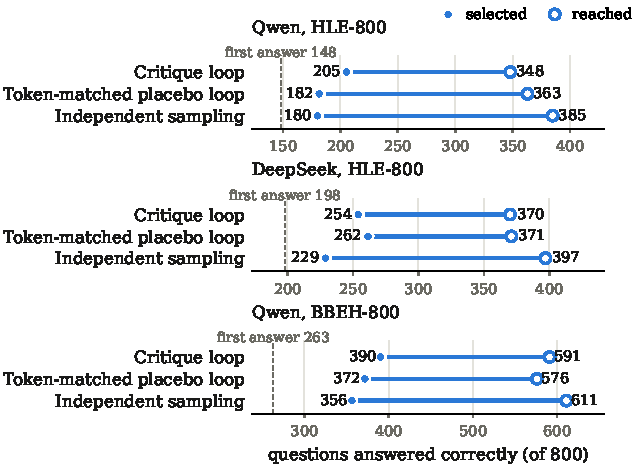
\includegraphics[width=\columnwidth]{figs/equal_tokens.pdf}
  \caption{Three methods given the same tokens. Open circle: questions \emph{reached} (a correct answer appears among the method's answers). Filled circle: questions \emph{selected} (the most frequent answer is correct). Reach is similar across methods and highest for independent sampling. The critique loop selects more than independent sampling in every panel. Exact counts and tests are in Table~\ref{tab:core}.}
  \label{fig:equal}
\end{figure}

\section{Related Work}

\paragraph{Reaching and selecting.}
We take the distinction between reaching and selecting from work on sampling.
\citet{brown2024monkeys} separate \emph{coverage}, meaning that some sample is correct, from picking the correct sample, and show that coverage keeps rising with more samples.
Majority voting does not keep pace with it \citep{chen2024morecalls}, and \citet{jain2026cliff} finds on competition mathematics that models pick the correct answer far less often than their samples contain it.
These studies concern independent sampling.
We apply the same two measures to a loop and to its controls, and our second finding is the loop-side counterpart of theirs: a loop narrows the gap between what is reached and what is selected.

\paragraph{Self-critique against independent sampling.}
Self-Refine and Reflexion introduced loops in which one model generates feedback for itself \citep{madaan2023selfrefine,shinn2023reflexion}.
Later comparisons are less favourable.
\citet{huang2024cannot} find that the gains of such loops largely vanish once the loop receives no hint about the correct answer, a condition our loops satisfy by design.
At equal cost, majority voting over samples is reported to match or beat reflection, debate and sequential revision \citep{wang2024token,wang2025rethinking,mirzaei2026sample}, and the gains of multi-agent debate are attributed largely to its final vote \citep{du2024debate,smit2024mad,choi2025debate}.
These results appear to contradict our second finding.
They differ from our setting in two ways that our data show to matter (Section~\ref{sec:equal}).
They read a loop by its last answer, where we read it by its most frequent answer, and their tasks have short answers in a fixed form, where our advantage lies on open-form answers.
\citet{snell2024scaling} show that the best split of a budget between parallel samples and sequential revisions depends on difficulty, which is one reason we restrict our claims to hard questions.

\paragraph{Placebo controls.}
That contentless doubt changes answers is known: asked ``Are you sure?'', models often give up a correct answer \citep{laban2024flipflop}.
Placebo feedback has been used as a control in code repair, where it is hard to beat and where studies disagree on whether the content of feedback matters \citep{olausson2024selfrepair,iscan2026falsification,iscan2026form,verma2026blind}.
Our third finding agrees with that picture and adds that the answer depends on the model.
Closest to our design, \citet{ning2026revision} use content-free drafts to split the gain of one model revising another's draft into re-solving, scaffold and content.
They measure final accuracy in a single pass through two models.
We iterate one model, match tokens across methods, and measure reach and selection separately.

\section{Setup}
\label{sec:setup}

\paragraph{The loop.}
A \emph{solver} answers each question once at temperature 0. We call this the \emph{first answer}.
In each later round the solver sees the question, its previous answer and a feedback message, and answers again. It is told to keep its answer if it believes the answer is correct.
The loop stops when the solver has given the same answer three times in a row, or after ten rounds of feedback.
All loops of a model start from the same first answer and differ only in the feedback (Table~\ref{tab:conditions}).

\paragraph{Critique loop.}
The feedback is written by a \emph{critic}, a separate call to the same model.
The critic reads the question, the current answer and the end of the solver's reasoning, and returns one to three doubts, each with a check the solver can carry out. It may not name an answer.

\paragraph{Placebo loops.}
In the \emph{reassuring loop} the feedback is always ``No confident error direction was found for this answer.''
In the \emph{generic-doubt loop} the feedback is one to three doubts in the critic's format, drawn from five fixed sentences such as ``you may have discounted a constraint stated in the problem'' (Appendix~\ref{app:prompts} gives the sentences and their origin).
No model is called to produce either.
A critique differs from generic doubt in more than content: it is longer, new in every round, and costs a model call. When we attribute an effect to the critique, we mean this whole package.

\paragraph{Independent sampling.}
The model answers the question repeatedly with the first-answer prompt at temperature 0.7.
The samples are combined in two ways: by taking the most frequent answer \citep{wang2023selfconsistency}, or by showing all samples to the model and asking which is most consistent with the others, known as universal self-consistency (USC) \citep{chen2023usc}.

\paragraph{Equal tokens.}
The critique loop sets the budget: on each question, the tokens its solver and critic spent (prompt plus completion, reasoning included).
A placebo loop that stops by itself spends less. The \emph{token-matched placebo loop} is therefore the generic-doubt loop with the stopping rule removed, run on each question until it has spent the budget.
Independent sampling likewise continues on each question until the samples have spent the budget, which gives 17 to 21 samples per question.

\begin{table}[t]
\centering
\small
\setlength{\tabcolsep}{3pt}
\begin{tabular}{@{}p{2.55cm}p{4.6cm}@{}}
\toprule
Method & What the solver receives or does \\
\midrule
Critique loop & 1--3 doubts by a critic that read the answer \\
Reassuring loop & ``no problem found'' \\
Generic-doubt loop & 1--3 fixed sentences, the same for all questions \\
Token-matched placebo loop & the generic-doubt loop, run to the critique loop's tokens \\
Independent sampling & separate answers at temperature 0.7, up to the critique loop's tokens \\
\bottomrule
\end{tabular}
\caption{Methods. The loops share the first answer and differ only in the feedback.}
\label{tab:conditions}
\end{table}

\paragraph{Data and models.}
Table~\ref{tab:studies} lists the four sets of questions.
\emph{HLE-400} is a sample of 400 text-only questions of Humanity's Last Exam (HLE) \citep{phan2025hle}, stratified by subject. Three models from three providers ran on it: deepseek-v4-flash (\ds), qwen3.8-flash (\qw) and MiniMax-M2.5 (\mm). Its results formed our hypotheses.
\emph{HLE-800} is a second sample of 800 questions, drawn by the same rule after the first and with no overlap. \qw{} and \ds{} ran on it. \mm{} did not, because of its cost and rate limits.
\emph{BBEH-800} consists of 80 questions from each of the ten tasks of BIG-Bench Extra Hard (BBEH) \citep{kazemi2025bbeh} on which \qw's first answers were correct 10\% to 40\% of the time in a screening run. \emph{BBEH-240} consists of 80 questions from each of the three tasks on which they were correct more than 80\% of the time (Appendix~\ref{app:bbeh}). \qw{} ran on both.
Our claims are about hard questions: first answers are correct on 19\% and 25\% of HLE-800 and on 33\% of BBEH-800.
Every call may use 16{,}384 tokens of reasoning and 8{,}192 of visible output.

\begin{table}[t]
\centering
\small
\setlength{\tabcolsep}{3pt}
\begin{tabular}{@{}l l l@{}}
\toprule
Questions & Models & Role \\
\midrule
HLE-400 & three models & hypotheses \\
HLE-800 & \qw, \ds & tests \\
BBEH-800 (hard) & \qw & tests \\
BBEH-240 (easy) & \qw & contrast \\
\bottomrule
\end{tabular}
\caption{The four sets of questions. Every test cited as confirmed was fixed, with its criterion, before its outcomes were computed (Appendix~\ref{app:order}).}
\label{tab:studies}
\end{table}

\paragraph{Scoring.}
Answers on HLE are free-form, and many correct answers cannot be recognized by string matching.
An answer is therefore first compared with the reference by exact matching after normalization. If it does not match, a \emph{grader} decides whether it states the same final answer as the reference.
The grader is gpt-6-astra, a model from a provider other than those of the solvers, which avoids a model grading its own family's output.
Identical answers receive identical grades in every method, and every comparison on HLE is repeated with exact matching alone.
On BBEH answers are scored by the benchmark's own rule-based scorer.
An answer that is cut off at the token limit before it is complete counts as incorrect.
Appendices~\ref{app:scoring} and~\ref{app:audit} give the protocol and a human audit of the scoring.

\paragraph{Outcomes.}
Every outcome is computed from the list of answers that a method gives to a question.
For a loop the list holds the first answer and the answers of all later rounds. For independent sampling it holds the samples.
A question is \emph{reached} if some answer in the list is correct, and \emph{selected} if the most frequent answer in the list is correct.
We read every method by its most frequent answer so that loops and sampling are treated alike. A loop could also be read by its last answer, which we report separately.
When several answers tie for most frequent, each is taken with equal probability and the question is scored by the expected value, so counts of selected questions can be fractional (Appendix~\ref{app:scoring}).
We call selected divided by reached the \emph{conversion} of a method.

\paragraph{Statistics.}
For reached questions we use exact McNemar tests.
For selected questions we use a paired permutation test over questions and report 95\% bootstrap intervals in brackets.
Two methods are called equivalent in reach when the 90\% interval of their difference lies within a margin fixed in advance, which is the standard two one-sided tests at the 5\% level.
Tests fixed in advance as a family are corrected by Holm's method, and ``significant'' means $p<0.05$ after that correction.

\paragraph{What was fixed in advance.}
Each test on HLE-800 and BBEH-800 was written down with its criterion before its outcomes were computed, and was computed with a script frozen beforehand.
The specifications and scripts are recorded with time-stamped commits in the project repository. They were not entered in an external registry.
We call these tests \emph{confirmatory} and everything else \emph{descriptive}.
Appendix~\ref{app:order} lists every test, its outcome and the departures from the plan.

\section{Results}

\subsection{The starting observation}
\label{sec:first}

On HLE-400 the critique loop, stopping by itself, was compared with the two other kinds of method (Appendix~\ref{app:first}).
Against independent sampling with nine samples, which cost about as much, it reached a similar number of questions and selected more ($+20.7$, $+23.1$ and $+12.2$ of 400 on the three models).
Against the reassuring loop it reached far more questions (198 against 153, 182 against 123 and 152 against 125, all significant) and selected only somewhat more ($+12.4$, $+23.3$ and $+5.2$, significant on \qw{} alone), while spending about twice the tokens.
Two questions followed.
Is the critique loop's greater reach over a placebo loop due to the critique or to the tokens?
And is its better selection over independent sampling due to the critique or to the loop?
The three findings below answer them on HLE-800 and BBEH-800.

\subsection{Tokens buy reach}
\label{sec:tokens}

\emph{Given the same tokens, no method reaches reliably more questions than another.}

\paragraph{Critique loop and placebo loop.}
On HLE-800 the critique loop and the token-matched placebo loop are equivalent in reach on both models: the differences are $-15$ questions on \qw{} and $-1$ on \ds, within the margins fixed in advance.
On BBEH-800 the difference is $+15$, which neither meets nor violates the margin.
On HLE-400 the same pattern had appeared: 182 against 181 questions on \qw{} and 152 against 156 on \mm, where the generic-doubt loop stopping by itself had reached only 149 and 128.
The extra questions that a critique loop reaches at its natural stop are therefore paid for by its tokens, not by the content of its critique.

\paragraph{Critique loop and independent sampling.}
Counting the samples that fit within the budget, independent sampling reaches about as many questions as the critique loop: 17 and 8 more on HLE-800 and 3 fewer on BBEH-800, none of them a significant difference.

\paragraph{A limit.}
Tokens alone are not quite enough.
On HLE-400 a reassuring loop continued to the same tokens still reached 23 fewer questions than the critique loop, a significant difference, while generic doubt and a critique written without seeing the answer came within three questions (Appendix~\ref{app:controls}).
Reach needs tokens and feedback that makes the solver try another answer. It does not need a critique of the answer.

\subsection{A loop buys selection}
\label{sec:equal}

\begin{table*}[t]
\centering
\small
\setlength{\tabcolsep}{4pt}
\begin{tabular}{@{}l ccc@{}}
\toprule
 & \qw, HLE-800 & \ds, HLE-800 & \qw, BBEH-800 \\
\midrule
Reached: critique loop / indep.\ sampling & 348 / \textbf{385} & 370 / \textbf{397} & 591 / \textbf{611} \\
Selected: critique loop / indep.\ sampling & \textbf{205.3} / 180.0 & \textbf{254.2} / 229.0 & \textbf{390.5} / 356.5 \\
Samples per question & 18.8 & 17.2 & 21.2 \\
\midrule
Selected, critique loop $-$ indep.\ sampling & $+25.3$ \ci{4.4}{46.5}$^{*}$ & $+25.2$ \ci{7.8}{41.8}$^{**}$ & $+34.0$ \ci{13.8}{55.0}$^{**}$ \\
\quad on questions both reach & $+26.8$ \ci{9.0}{44.9}$^{**}$ & $+32.0$ \ci{17.6}{46.4}$^{***}$ & $+35.4$ \ci{16.0}{54.0}$^{**}$ \\
Selected, critique loop $-$ USC & $+22.3$ \ci{1.5}{43.1}$^{*}$ & $+19.2$ \ci{2.0}{37.1}$^{*}$ & -- \\
\bottomrule
\end{tabular}
\caption{The critique loop against independent sampling at equal tokens. The lower rows are confirmatory tests, with $p$ after Holm's correction within each column ($^{*}p<0.05$, $^{**}p<0.01$, $^{***}p<0.001$). Independent sampling keeps the sample that crosses the budget and so spends 13\% to 18\% more tokens than the critique loop. Both methods reach 290, 323 and 540 questions.}
\label{tab:core}
\end{table*}

\emph{At equal tokens the critique loop selects significantly more questions than independent sampling, in all three settings} (Table~\ref{tab:core}).
The differences are 25.3 and 25.2 questions of 800 on HLE-800 and 34.0 on BBEH-800, which is 14\%, 11\% and 10\% more than independent sampling selects.
The difference is as large or larger on the questions that both methods reach, so it is not a matter of which questions are reached.
On HLE-800 the critique loop also selects significantly more than USC, in which the model itself picks the consensus among the samples.

\textbf{More independent sampling buys reach and almost no selection.}
Going from nine samples to the token-matched number, independent sampling reaches 56, 36 and 64 more questions and selects only 1.9, 4.4 and 12.0 more.
Of every 100 questions it reaches, independent sampling selects 47, 58 and 58. The critique loop selects 59, 69 and 66.

\paragraph{Robustness.}
The result does not depend on the grader: with exact matching alone the differences on HLE-800 are $+28.6$ and $+17.2$, with intervals that exclude zero, and on BBEH-800 no grader is involved.
It does not depend on the loop's list containing the first answer, or on independent sampling spending slightly more: without the first answer the differences are 29.1, 26.5 and 39.7, and with the samples held within the budget they are 28.5, 26.4 and 52.5.
On HLE-400, where nine samples cost about as much as the critique loop (84\% to 112\% of its tokens), the critique loop also selected more on all three models, including \mm{} ($+12.2$, \ci{1.0}{24.0}). Those questions formed the hypothesis, so we do not count them as a test.

\paragraph{Scope.}
Three descriptive analyses mark where the advantage holds (Appendix~\ref{app:e2}).
\emph{Answer format.} On HLE-800 the advantage lies on the 599 open-form questions ($+24.3$ and $+19.8$). On the 201 multiple-choice questions it is small ($+1.0$ and $+5.4$).
\emph{Last answer.} If the loop is read by its last answer, the advantage is unchanged on HLE-800 ($+27.0$ and $+25.0$) and disappears on BBEH-800 ($+0.5$). On BBEH-800 a loop must be read by its most frequent answer.
\emph{Spelling.} Independent sampling may write one correct answer in several ways and so split its count. If all correct answers to a question are counted as one, which favours independent sampling because it uses the reference answer, the critique loop remains clearly ahead on \ds{} ($+19.2$, \ci{2.8}{36.5}) and on BBEH-800 ($+27.3$, \ci{7.2}{49.4}) but not on \qw{} with HLE-800 ($+9.3$, \ci{-13.3}{31.5}). In that setting part of the advantage may come from the loop writing its answer the same way each time.

\subsection{The critique is not always needed}
\label{sec:placebo}

\begin{table}[t]
\centering
\small
\setlength{\tabcolsep}{2.4pt}
\begin{tabular}{@{}l ccc@{}}
\toprule
 & \qw, & \ds, & \qw, \\
 & HLE-800 & HLE-800 & BBEH-800 \\
\midrule
\multicolumn{4}{@{}l}{\emph{Selected, critique loop minus}} \\
Token-matched & $\mathbf{+23.8}$ & $-7.2$ & $+18.6$ \\
\quad placebo loop & \ci{5.9}{42.3} & \ci{-23.9}{9.3} & \ci{-3.3}{41.4} \\
Reassuring loop & $\mathbf{+36.8}$ & $-1.9$ & $+10.6$ \\
 & \ci{17.4}{57.3} & \ci{-18.6}{15.3} & \ci{-11.3}{33.5} \\
\bottomrule
\end{tabular}
\caption{The critique loop against placebo loops. Both comparisons were confirmatory in each column (bold: significant after Holm's correction). The reassuring loop stops by itself and spends 37\% to 50\% of the critique loop's tokens.}
\label{tab:placebo}
\end{table}

\emph{Whether the loop needs a critique in order to select well depends on the model} (Table~\ref{tab:placebo}).

\paragraph{\qw{} on HLE-800: the critique is needed.}
The critique loop selects significantly more questions than the token-matched placebo loop ($+23.8$) and than the reassuring loop ($+36.8$).
A placebo loop with the critique loop's tokens selects no more than independent sampling ($+1.5$, \ci{-13.5}{16.5}).

\paragraph{\ds{} on HLE-800: the critique is not needed.}
Neither test is significant, and the estimates are close to zero.
The reassuring loop, which only ever tells the solver that no problem was found, selects 256.2 questions against 254.2 for the critique loop while spending 37\% of its tokens.
It selects 27.1 more than independent sampling (\ci{8.6}{45.0}).
For this model the gain in selection comes from being asked again.

\paragraph{\qw{} on BBEH-800: undecided.}
The critique loop is ahead of the two placebo loops by 18.6 and 10.6 questions, and neither difference is significant.

\paragraph{Temperature.}
The loops answer at temperature 0 and independent sampling at 0.7, so the loop's advantage might come from temperature.
On BBEH-800 we ran the token-matched placebo loop at temperature 0.7.
Its selected count barely changed (368.0 against 371.9 at temperature 0), which speaks against temperature as the cause.
It remained ahead of independent sampling, though not significantly ($+11.6$, \ci{-9.6}{31.6}), so we cannot rule temperature out for a loop without a critique.

\subsection{Why a loop selects better}
\label{sec:mech}

The analyses in this section were not fixed in advance. We offer them as an explanation, not as a result.

\paragraph{The critic does not know which answers are correct.}
The critic raises as many doubts about a correct answer as about an incorrect one: 2.96 against 2.96 per round on \qw, 2.81 against 2.86 on \ds{} and 2.94 against 2.95 on BBEH-800.

\paragraph{The solver gives up incorrect answers more readily.}
Table~\ref{tab:keep} gives the probability that the solver keeps its answer in the next round.
In every method a correct answer is kept more often than an incorrect one.
Under critique the difference is largest: an incorrect answer is kept in only 29\%, 29\% and 16\% of rounds.
The critique loop thus acts as a filter. It keeps the solver moving, incorrect answers are abandoned sooner than correct ones, and correct answers end up as the most frequent.
Independent sampling has no such filter. Its samples do not see each other and spread over nearly twice as many distinct answers (6.0 to 6.6 per question on HLE-800, against 3.3 and 3.4 for the critique loop).
On \ds{} the solver filters well enough under mere reassurance, which is why the critique adds nothing there.

\begin{table}[t]
\centering
\small
\setlength{\tabcolsep}{2.1pt}
\begin{tabular}{@{}l cc c cc c cc@{}}
\toprule
 & \multicolumn{2}{c}{\qw} & & \multicolumn{2}{c}{\ds} & & \multicolumn{2}{c}{\qw} \\
 & \multicolumn{2}{c}{HLE-800} & & \multicolumn{2}{c}{HLE-800} & & \multicolumn{2}{c}{BBEH-800} \\
\cmidrule(lr){2-3}\cmidrule(lr){5-6}\cmidrule(l){8-9}
 & cor. & inc. & & cor. & inc. & & cor. & inc. \\
\midrule
Reassuring loop & .64 & .60 & & .75 & .63 & & .72 & .38 \\
Token-matched & .58 & .54 & & .73 & .61 & & .70 & .49 \\
Critique loop & .43 & \textbf{.29} & & .44 & \textbf{.29} & & .45 & \textbf{.16} \\
Indep.\ sampling & .35 & .31 & & .50 & .34 & & .58 & .32 \\
\bottomrule
\end{tabular}
\caption{Probability that the next answer repeats the current one, when the current answer is correct (cor.) or incorrect (inc.). For independent sampling (nine samples): the probability that two consecutive samples agree. Descriptive.}
\label{tab:keep}
\end{table}

\paragraph{Two tests of this explanation.}
If a loop selects well because the solver sees its previous answer, hiding that answer should lower what the loop selects.
On BBEH-800 it did, by 12.4 questions, but the difference was not significant (\ci{-6.0}{30.9}; Appendix~\ref{app:memory}).
We also predicted that the critique loop's gain would be largest on questions where the model is unsure of its first answer and that answer is wrong. The gain was spread more widely than predicted (Appendix~\ref{app:bbeh}).
The explanation is therefore consistent with the data and not established.

\section{Discussion}

\paragraph{What is established.}
Three conclusions rest on tests fixed in advance, all on hard questions.
\emph{Tokens buy reach.} With the same tokens, a critique loop reaches no more questions than a placebo loop (two models on HLE-800).
\emph{A loop buys selection.} With the same tokens, a critique loop selects more questions than independent sampling, whether the samples are combined by their most frequent answer or by the model's own choice of consensus (two models on HLE-800, one on BBEH-800).
\emph{The critique is not always needed.} Its contribution to selection is established for one model and absent for the other.

\paragraph{What a critique is for.}
Reach and selection have different sources.
Reach comes from spending tokens on new answers, and independent sampling does this at least as well as a loop.
Selection comes from the loop.
The critic cannot tell correct answers from incorrect ones, but being asked again makes the solver give up incorrect answers more readily than correct ones, and so correct answers accumulate.
A critique strengthens this filter on a model that would otherwise repeat its answer whatever its merit, as \qw{} does under reassurance.
On a model whose answers already sort themselves when it is asked again, as on \ds, the critique adds cost and nothing else.

\paragraph{Earlier results.}
Studies that find majority voting over samples ahead of sequential revision \citep{wang2025rethinking,mirzaei2026sample} read a loop by its last answer and use tasks whose answers are short and fixed in form.
Our scope analyses show both conditions to matter: the loop's advantage lies on open-form answers, and on BBEH-800 it requires reading the loop by its most frequent answer.
The two sets of results are compatible, and the conditions under which each holds are part of the finding.

\paragraph{Use.}
When answers can be checked from outside, by a test, a tool or a trusted verifier, reach is what matters, and independent sampling provides it as cheaply as a loop and in parallel.
When nothing outside the model can check an answer, selection is what matters, and a loop selects better than independent sampling at the same cost.
The cheapest loop is worth trying first: on one of our two models, asking again with ``no problem found'' selected as well as a critique loop that cost almost three times as much.

\paragraph{The remaining gap.}
Every method leaves many reached questions unselected: 116 to 201 of the questions that the critique loop reaches.
We conjecture that closing this gap is a matter of the model and not of the loop. A loop can only exploit the model's own tendency to hold on to correct answers more firmly than to incorrect ones, and that tendency is set in training.
Appendix~\ref{app:props} describes three properties of a model that could be measured to test this.

\section{Conclusion}

We compared a self-critique loop with placebo loops and with independent sampling at equal tokens, and measured separately what each method reaches and what it selects.
Tokens buy reach: with the same tokens the three methods reach about the same number of questions.
A loop buys selection: the critique loop selects more questions than independent sampling on two models and two benchmarks.
The critique is not always needed: on one model a loop that merely asks again selects as well.
On hard questions the value of self-critique is in settling on the right answer, not in finding it.

\section*{Limitations}

\paragraph{Scope.}
Our conclusions are about hard questions, on which first answers are mostly wrong (19\% to 33\% correct). On the easy tasks of BBEH no loop changes much (Appendix~\ref{app:bbeh}).
The models are three models of one price tier, with one model as both solver and critic. \mm{} was run on HLE-400 only, and only \qw{} was run on BBEH.
Stronger models, critics stronger than the solver, and tasks with an executable check may behave differently.

\paragraph{Design.}
Loops answer at temperature 0 and independent sampling at 0.7. Raising a placebo loop's temperature changed little, but we did not run a critique loop at temperature 0.7.
We read a loop by its most frequent answer. Read by its last answer, the critique loop keeps its advantage over independent sampling on HLE-800 and loses it on BBEH-800.
On \qw{} with HLE-800 part of the advantage may come from consistent spelling of answers (Section~\ref{sec:equal}).
The explanation in Section~\ref{sec:mech} is descriptive. Two attempts to test it directly did not reach significance.
The question-only critic used in one control on HLE-400 often solves the question itself, so that control does not remove answer information from the feedback (Appendix~\ref{app:controls}).

\paragraph{Scoring.}
HLE answers are free-form, so exact matching misses many correct answers and a grader model decides the rest, about a third of the answers scored correct.
All comparisons on HLE were repeated with exact matching alone and lead to the same conclusions. A human audit of 100 scored answers agreed with the automatic scoring on 93 (Appendix~\ref{app:audit}).
Some reference answers of HLE are wrong \citep{zhai2026hleverified}, which affects every method alike.
Each method was run once per model. A repeat of two methods on 400 questions moved their selected counts by 2.7 and 4.4, variation that intervals over questions do not capture.

\paragraph{Process.}
The tests were fixed before the runs and recorded in a version-controlled repository, not in an external registry.
The confirmation on HLE-800 began with \qw, chosen because its effect was clearest on HLE-400.
Appendix~\ref{app:order} lists the departures from the plan.

\section*{Ethics Statement}

The study uses public benchmarks and commercial model interfaces.
Two people checked samples of scored answers and of critiques. No personal data were collected.
We see no specific risk beyond those of the underlying models.

\section*{Use of AI Assistants}

The authors chose the research questions, decided on the designs, the protocols and the claims, and are responsible for the content of the paper.
AI assistants were used extensively under the authors' direction.
An AI assistant (Claude, Anthropic) drafted the experiment specifications, which the authors revised and approved before the runs, wrote the analysis code, and drafted and revised the text. A separate AI coding agent executed the runs.
In the audits, the same assistant wrote notes or reviewed human labels, as described in Appendices~\ref{app:audit} and~\ref{app:controls}.
Every number in the paper is produced from the frozen outputs by a script in the accompanying repository and is checked automatically against the text. The main tests were recomputed with a standard statistics library (SciPy) with identical results up to Monte Carlo error.

\bibliography{refs}

\appendix

\section{Methods and Prompts}
\label{app:prompts}

All answers, per-answer scores, judge verdicts and analysis code are released with the paper.

\paragraph{Solver.}
The first answer uses the benchmark prompt.
In later rounds the solver receives the question again with this message: ``A reviewer looked at your PREVIOUS answer to this question and gave feedback. Your previous answer was: [answer]. Reviewer feedback: [feedback]. Reconsider the question and provide your final answer again. If you believe your previous answer was already correct, keep it as is.''
Each round is a separate call. No conversation history is carried over.

\paragraph{Reassuring loop.}
The feedback is the fixed sentence ``No confident error direction was found for this answer.''

\paragraph{Critique loop.}
The critic's system prompt states that it inspects a committed answer to a hard question and identifies the most likely wrong directions. That it never reads the reference answer, never gives a probability, never names the correct answer or any answer content, and speaks only of possibilities.
The user message contains the question, the answer and the last 6{,}000 characters of the solver's reasoning.
The critic returns one to three doubts, each with a short label, a suspicion about this answer's specific shortcoming, and a check that the solver can run without the reference answer. It is told not to derive or solve the question again.
The critic returned three doubts in 86\% of rounds on \ds, 95\% on \qw{} and 66\% on \mm.
If the critic fails twice, the round uses the reassuring sentence (30 of 2{,}358 rounds on \ds, 10 on \qw, 4 on \mm).

\paragraph{Generic-doubt loop.}
Each round draws a number of doubts $k\in\{3,2,1\}$ with probabilities 0.86, 0.11 and 0.03, the distribution observed for the critic on \ds{} and used for all models, and then $k$ of five generic sentences without replacement, seeded by the question identifier and the round.
Each is rendered as ``[name]: you may have [generic suspicion]. To check: [generic check].'', for example ``constraint-blind decimation: you may have discounted a constraint or condition stated in the problem. To check: re-read the problem statement, list every stated constraint, and confirm the answer satisfies each one.''
The five sentences are named after the error types of Appendix~\ref{app:bank}.

\paragraph{Independent samples and USC.}
Samples use the prompt of the first answer at temperature 0.7. For the comparisons at equal tokens they are continued as described in Appendix~\ref{app:e2}. USC uses the prompt of \citet{chen2023usc}: the model receives all responses to a question, numbered, and must end with ``The most consistent response is Response N''.
Sampling does not lower the quality of single answers: one sample is correct on 117, 80 and 82 questions on average, against 113, 69 and 81 for the first answer.

\section{The Restricted Critic}
\label{app:bank}

The study began with a critic that must choose each doubt from a list of five error types.
The list was distilled from 33 incorrect answers of deepseek-v4-flash on six other benchmarks (GPQA-Diamond, MMLU-Pro, MATH-500, BFCL, BBH and AIME): constraint-blind decimation; descriptor or label conflation; procedure truncation or omission; retrieval abort; format or precision non-conformance.
No question or answer from Humanity's Last Exam enters the list.
The critique loop of the main text, whose critic is free to name the shortcoming itself, was introduced as a control for this list.

On \ds{} the restricted critic gives last 140, selected 150.9 and reached 192, against 148, 157.4 and 198 for the critique loop. The differences are not significant (reached 23/17; selected $+6.5$, \ci{-6.4}{18.9}).
We had fixed in advance that the list would be judged to have no identifiable effect if the unrestricted critic reached at most five questions fewer. It reaches six more.
The restricted critic was not run on the other models, and the main text uses the unrestricted critic throughout.
Against the two placebo loops the restricted critic's selected questions differ by $+5.9$ (\ci{-6.8}{18.5}) and $+4.8$ (\ci{-6.5}{16.4}). Against nine samples by $+14.1$ (\ci{2.5}{26.7}).

\section{Scoring Protocol}
\label{app:scoring}

This appendix describes the scoring on HLE. Differences reported throughout the paper are computed from unrounded counts and can differ by 0.1 from differences of the rounded counts. On BBEH every answer is scored by the benchmark's own rule-based scorer, used unchanged, and no model is involved (Appendix~\ref{app:bbeh}).

\paragraph{Steps.}
(1) An answer whose generation was cut off at the token limit is incorrect.
(2) Otherwise the answer is matched against the reference by rules that depend on the answer type (option letter, integer, normalized string).
(3) Unmatched answers are graded once by a model from a different provider (gpt-6-astra), the grader. The grade is stored per question and answer, so identical answers receive identical verdicts in all methods.
(4) On \ds, answers on which the grader and a second model-based check disagreed were graded three more times and decided per answer variant. The resulting rules are applied wherever the same variant recurs, on all models.
Of the answers scored correct, about six in ten are exact matches and four in ten are accepted in steps (3) or (4).

\paragraph{Candidates and ties.}
A candidate is correct if its last occurrence is scored correct.
Occurrences of one candidate usually share a grade. They can differ when one occurrence was cut off at the token limit, or when two strings that normalize to the same candidate were graded differently (5 of 3{,}251 candidates on \mm).
Under the alternative rule that resolves ties in favour of the more recent answer, which is available to loops and not to samples, the selected counts on \ds{} are 144, 147 and 159 for the reassuring, generic-doubt and critique loops, against 145.0, 146.1 and 157.4 under random ties.

\paragraph{Failed calls and truncation.}
Any loop containing a failed call was rerun in full: on \ds{} 29 questions for the generic-doubt loop and one to four for the other methods. On \qw{} 61 first answers with the loops that depend on them. None on \mm.
An error message never counts as an answer.

\paragraph{A grading incident.}
After the confirmation on \ds{} had been read, a check by the authors found that the share of answers accepted by the grader on \ds's HLE-800 questions was far below that on the first questions (2\% to 3\% against 15\% to 16\%). In the grader's cache, 8{,}106 of 18{,}874 entries were interface errors (for example, permission denied) that had been stored as ``incorrect''. Three score files were affected: \ds{} on HLE-800, the added \qw{} runs (nine samples and the question-only critique) and the repeated runs. The file behind the first confirmation on \qw{} was not. All read-outs that used the affected files were voided, every affected answer was graded again, a script that checks every graded round for a real verdict was added and is run before every read-out, and the voided read-outs were repeated once with unchanged scripts. The conclusions about \ds's placebo comparisons did not change. Its comparison with nine samples became confirmed. We report only the repeated read-outs.

\paragraph{Two spellings, two verdicts.}
The grader judges the raw answer while votes are counted by normalized candidate, so two spellings of one candidate can receive different verdicts. Among the candidates of the critique loop, the reassuring loop, the token-matched loop and the samples at equal tokens taken together, this happens for 20 of 8{,}664 on \qw{} and 19 of 8{,}464 on \ds, each on a different question. Resolving them by majority, by `correct if any' or by `correct only if all' gives critique minus samples of $+27.3$, $+27.8$ and $+27.8$ on \qw{} and $+25.7$, $+24.7$ and $+23.7$ on \ds, against $+25.3$ and $+25.2$ as scored. Every interval excludes zero.
On \ds{} between 6.4\% and 8.0\% of rounds per method are cut off at the token limit, including 28 first answers. On \qw{} one round. On \mm{} at most 0.9\% per method.

\section{Audit of the Scoring}
\label{app:audit}

We drew 100 scored answers, stratified by model, method and scoring step, and hid the model, the method and the automatic verdict.
Before any formal annotation we fixed three ways of handling an answer, according to what a comparison with the reference requires.
The first is a human judgement made without any model. The third is a human judgement made with model-written notes in view.

\emph{Direct comparison} (66 answers: option letters, numbers, short strings).
One annotator judged each answer as correct, incorrect or unsure without using a language model, and a second person reviewed the judgements. Because the reviewer saw some of the first annotator's labels, we report no agreement statistic between them.
On 53 answers the judgement was definite and stood. All 53 agree with the automatic verdict.
The other 13 went to discussion: seven that the annotators judged incorrect although the automatic scoring had accepted them, five marked unsure, and one on which annotator and reviewer differed.

\emph{Symbolic check} (12 answers: two mathematical expressions).
Both expressions were transcribed for a computer algebra system and compared symbolically and numerically. An annotator confirmed the transcriptions.
All 12 are equivalent, and all 12 had been accepted by the automatic scoring.

\emph{Discussed adjudication} (35 answers: 22 that require reading the question closely, such as answers conditional on a convention, and the 13 from direct comparison).
For each answer a language model that is neither a solver nor the grader (Claude, Anthropic; model identifier claude-fable-5-2) wrote a note that states the point to be decided and, in 32 cases, suggests a verdict. The notes were written without access to the automatic verdict for 16 of the 35 answers.
A human adjudicator then decided each case with the note in view.
On the 32 answers for which the note suggests a verdict, the adjudicator's decision coincides with the suggestion. On the three for which it does not (an alternative construction that could not be verified, and two unevaluated expressions) the adjudicator decided that the answer is incorrect.
This part of the audit is therefore human adjudication assisted by a model, and its decisions are not independent of the notes.
Three items of one question were checked by exhaustive computation, and numerical answers were held to one rule: an answer is correct if it equals the reference rounded to the answer's own number of significant digits.
The seven answers that the annotators had rejected in direct comparison were decided as follows: five are the same answer in another notation or become identical under a formatting rule stated in the question, one agrees with the reference after rounding, and one does not.

\emph{Result.}
The audit agrees with the automatic scoring on 93 of the 100 answers (53 of 53, 12 of 12 and 28 of 35 in the three parts).
Of 71 answers that the automatic scoring accepted, six were judged incorrect: four of the 62 accepted by the grader, two of the four accepted through adjudication, and none of the five exact matches.
Of 29 answers that it rejected, one was judged correct (an answer conditional on a sign convention that the question leaves open).
The six false acceptances are a rounded number that does not match, an answer less specific than the reference, two unevaluated expressions, an unverified alternative construction and a constraint system that the computation shows to be inexact.
They are not spread evenly: three fall among the four audited acceptances of the critique loop on \qw, and one each in the reassuring loop, the restricted critic and independent samples on \ds.
The sample is far too small to estimate an error rate per method, so the comparisons under exact matching (Section~\ref{sec:first}, Appendix~\ref{app:more}), which do not use the grader, remain the main safeguard.

\emph{A second audit.}
A second audit, of 100 answers behind the selected questions of three loops on HLE-800 with \qw{} (84 accepted and 16 rejected by the grader), follows the same three paths, fixed before any annotation: 60 answers for direct comparison by one annotator and one reviewer, 17 for a symbolic check (16 equivalent, one not), and 23 for discussion. Its annotation was not complete at the time of writing, and no claim in this paper depends on it. It does not cover independent samples, for which the comparisons under exact matching serve as the check.

\section{Order of the Studies and What Was Fixed in Advance}
\label{app:order}

Table~\ref{tab:order} lists every part of the study after the first one, with the tests fixed in advance and their outcomes.
For each part a written specification gave the conditions, the tests, their criteria and how each outcome would be read. The read-out script was committed with a recorded hash before it was run once on the scored data, and its output hash was recorded.
Specifications and scripts were never changed after a run began, with two exceptions noted below.
Before every full run, 16 questions were run and only run statistics were inspected (completion, cut-off answers, rounds, tokens). No correctness was computed.

\begin{table*}[t]
\centering
\small
\setlength{\tabcolsep}{3pt}
\begin{tabular}{@{}p{3.6cm} p{4.4cm} p{2.6cm} p{4.6cm}@{}}
\toprule
Part & Tests fixed in advance & Fixed & Outcome \\
\midrule
Controls, \qw, HLE-400 & reach: critique against token-matched, mismatched, question-only (Holm) & before the runs & no difference; difference; difference \\
Continuation to equal tokens, \qw, HLE-400 & reach: critique against continued reassuring, mismatched, question-only (Holm) & before the continuation & difference; not after correction; no difference \\
Confirmation, \qw, HLE-800 & selected: critique $-$ token-matched, critique $-$ reassuring (Holm); reach equivalence $\pm33$ & before the runs & both confirmed; equivalent by one question \\
Addendum, \qw, 800 new & selected: critique $-$ nine samples, critique $-$ question-only at equal tokens (Holm) & after the confirmation was read; before these runs & confirmed; not confirmed \\
Confirmation, \ds, HLE-800 & as for \qw, plus critique $-$ nine samples (Holm over three); reach equivalence $\pm27$ & before the runs & not, not, confirmed; equivalent \\
BBEH, \qw, 800 hard & as for \ds{} (Holm over three); reach equivalence $\pm33$; five predictions & before the runs; predictions before the read-out & not, not, confirmed; inconclusive; two predictions failed \\
Samples at equal tokens and USC, \qw{} and \ds, HLE-800 & selected: critique $-$ samples, critique $-$ USC; added: critique $-$ samples on questions both reach, reach equivalence & first two before the runs; last two after the runs, before scoring & all six selection tests confirmed; reach not equivalent \\
Removing the previous answer, \qw, BBEH & selected: with $-$ without the previous answer, after a check of the manipulation & before the runs & manipulation effective; not confirmed \\
Samples at equal tokens and temperature, \qw, BBEH & selected: critique $-$ samples; on questions both reach; loop at temperature 0.7 $-$ samples (Holm); reach equivalence & before the runs & confirmed, confirmed, not confirmed; not equivalent \\
\bottomrule
\end{tabular}
\caption{Parts of the study after the first, in the order in which they were run. All on HLE unless marked BBEH.}
\label{tab:order}
\end{table*}

\paragraph{Departures.}
(i) The confirmation on \qw{} did not include independent samples. They were added, with a test written before they were run, after the first tests of the confirmation had been read.
(ii) For the comparison at equal tokens on HLE, the tests on questions that both methods reach and on reach were written after the runs had finished and while the new samples were being scored, before any per-question count of reached or selected questions had been computed. The record notes that the scoring cache was being written at the time.
(iii) The grading incident of Appendix~\ref{app:scoring} voided three read-outs, which were repeated with unchanged scripts after the scores were repaired.
(iv) In one run the number of parallel requests exceeded the agreed limit. This affects only the speed of the run, and the checks of completeness found no effect.

\paragraph{The first study.}
The first study was run one model at a time. What was fixed before each model is listed in Appendix~\ref{app:prereg}.
Its single confirmatory test was not met.
The model for the confirmation, \qw, was chosen after the first study as the one whose gain over the reassuring loop excluded zero there. The confirmation asks whether that result holds on new questions, not whether it holds on a model taken at random.

\section{Analyses Fixed in Advance in the First Study}
\label{app:prereg}

Each item below was written down in a dated internal document before the corresponding data existed. None was registered externally.
The documents are part of the released material.

\emph{First model (\ds).}
(i) The most frequent answer of the critique loop against that of nine samples; written for the restricted critic of Appendix~\ref{app:bank}, which passes ($p=0.03$).
(ii) The unrestricted critic as a control for the list of error types, with the criterion given in Appendix~\ref{app:bank}.
(iii) The generic-doubt loop: critique content is judged effective if this loop reaches at least 15 questions fewer than the critique loop at $p<0.05$ (observed: 27 fewer).
(iv) The acceptance criteria for the judges of Appendix~\ref{app:judges}.
(v) Comparisons at equal token cost: the critique loop against a vote over eleven samples (holds) and against the model's own choice of consensus among eleven samples (interval includes zero).

\emph{Second model (\qw).}
Four tests: critique loop against nine samples on selected questions; reach of the critique loop against the reassuring loop; reach of the generic-doubt loop at least 15 below the critique loop; ratio of repeat probabilities in the critique loop above that in the reassuring loop.
All four hold.

\emph{Third model (\mm).}
One confirmatory test: the critique loop selects more questions than the reassuring loop (interval excludes zero).
The criterion is not met ($+5.2$, \ci{-6.9}{18.0}).
Secondary tests: the same against the generic-doubt loop (not met, $+4.6$, \ci{-8.4}{16.8}); reach of the critique loop against the reassuring loop (holds); reach of the generic-doubt loop at least 15 below the critique loop (holds, 24 below); reach of the generic-doubt loop above the reassuring loop (not met, 128 against 125); critique loop against nine samples on selected questions (holds by the stated criterion, interval \ci{1.0}{24.0}; permutation $p=0.051$); ratio of repeat probabilities (holds).
We had also fixed that, if the confirmatory test held, reach and selection would both be headline results, and that otherwise reach would be the only headline and the test would be reported as not met.
The model first chosen as the third model, glm-5.3, could not be run within the token allowance on a 16-question check of run health. Before any answer was scored it was replaced by MiniMax-M2.5, the first candidate from another provider to pass that check.

\emph{Controls on \qw} (after the main study).
Three primary tests on reach, each written down with the reading of every outcome before the runs and corrected together by Holm's method: the critique loop against the token-matched control (not significant), against the mismatched critique (significant) and against the question-only critique (significant); comparisons of selected questions were specified as descriptive (Appendix~\ref{app:controls}, which also lists two settings changed after a check of run health).

Two analyses were added after a review of a draft, with their rules written down before computing: reach by subject area, and results on the questions drawn first and last (Appendix~\ref{app:more}).
They and all other analyses are exploratory.
The random-tie convention replaced an earlier asymmetric one after internal review.

\section{HLE-400: Details}
\label{app:more}
\label{app:first}

Table~\ref{tab:main} and Figure~\ref{fig:first} give the outcomes of every method in the first study at its natural stop, and Table~\ref{tab:pairs} the paired comparisons.

\begin{figure}[h]
  \centering
  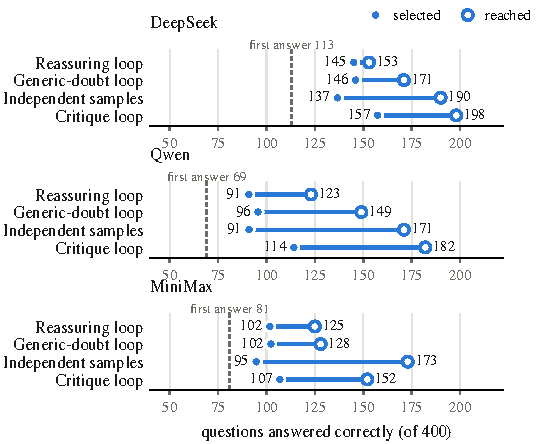
\includegraphics[width=\columnwidth]{figs/reach_select.pdf}
  \caption{First study: questions out of 400 that each method \emph{reaches} (a correct answer appears among its answers; open circle) and \emph{selects} (its most frequent answer is correct; filled circle). The dashed line marks the first answer, which all three loops share. At their natural stop the critique loop moves the open circle far more than the filled one. Tests and intervals are in Table~\ref{tab:pairs}.}
  \label{fig:first}
\end{figure}

\begin{table*}[t]
\centering
\small
\setlength{\tabcolsep}{3.4pt}
\begin{tabular}{@{}l rrrr c rrrr c rrrr@{}}
\toprule
 & \multicolumn{4}{c}{\ds{} (first answer 113)} & & \multicolumn{4}{c}{\qw{} (first answer 69)} & & \multicolumn{4}{c}{\mm{} (first answer 81)} \\
\cmidrule(lr){2-5}\cmidrule(lr){7-10}\cmidrule(l){12-15}
Method & Last & Sel. & Reached & Conv. & & Last & Sel. & Reached & Conv. & & Last & Sel. & Reached & Conv. \\
\midrule
Reassuring loop & 141 & 145.0 & 153 & \textbf{.95} & & 89 & 90.8 & 123 & \textbf{.74} & & 100 & 101.7 & 125 & \textbf{.81} \\
Generic-doubt loop & 142 & 146.1 & 171 & .85 & & 92 & 95.6 & 149 & .64 & & 101 & 102.3 & 128 & .80 \\
Critique loop & 148 & \textbf{157.4} & \textbf{198} & .79 & & 112 & \textbf{114.1} & \textbf{182} & .63 & & 99 & \textbf{106.9} & 152 & .70 \\
Independent samples & -- & 136.7 & 190 & .72 & & -- & 91.0 & 171 & .53 & & -- & 94.7 & \textbf{173} & .55 \\
\bottomrule
\end{tabular}
\caption{Questions answered correctly, out of 400, for three models. \emph{Last}: the loop's last answer is correct. \emph{Sel.}: selected. \emph{Conv.}: conversion, selected divided by reached. Conversion is an exploratory, descriptive ratio: methods reach different questions, so it compares different sets.}
\label{tab:main}
\end{table*}

\begin{table*}[t]
\centering
\fontsize{8}{9.6}\selectfont
\setlength{\tabcolsep}{1.5pt}
\begin{tabular}{@{}l ll c ll c ll c l@{}}
\toprule
 & \multicolumn{2}{c}{\ds} & & \multicolumn{2}{c}{\qw} & & \multicolumn{2}{c}{\mm} & & Mean of three \\
\cmidrule(lr){2-3}\cmidrule(lr){5-6}\cmidrule(lr){8-9}\cmidrule(l){11-11}
Comparison & Reached & Selected & & Reached & Selected & & Reached & Selected & & Selected \\
\midrule
Critique -- reassuring & 52/7$^{***}$ & $+12.4$ \ci{-1.6}{25.6} & & 69/10$^{***}$ & $+23.3$ \ci{8.8}{39.2} & & 38/11$^{***}$ & $\mathbf{+5.2}$ \ci{-6.9}{18.0}$^{\dagger}$ & & $+13.6$ \ci{5.1}{22.2} \\
Critique -- generic & 39/12$^{***}$ & $+11.3$ \ci{-0.8}{23.7} & & 49/16$^{***}$ & $+18.5$ \ci{3.9}{34.3} & & 37/13$^{***}$ & $+4.6$ \ci{-8.4}{16.8} & & $+11.5$ \ci{3.4}{20.1} \\
Generic -- reassuring & 28/10$^{**}$ & $+1.2$ \ci{-10.1}{12.5} & & 42/16$^{***}$ & $+4.8$ \ci{-8.1}{18.6} & & 21/18 & $+0.7$ \ci{-11.4}{12.8} & & $+2.2$ \ci{-5.2}{9.8} \\
Critique -- samples & 29/21 & $+20.7$ \ci{9.0}{32.4} & & 44/33 & $+23.1$ \ci{9.6}{38.6} & & 19/40$^{**}$ & $+12.2$ \ci{1.0}{24.0} & & $+18.7$ \ci{10.7}{26.4} \\
\bottomrule
\end{tabular}
\caption{Paired comparisons on the same 400 questions. \emph{Reached}: $a/b$ means that $a$ questions are reached only by the first method and $b$ only by the second (exact McNemar test; $^{**}p<0.01$, $^{***}p<0.001$). \emph{Selected}: difference in selected questions, first minus second, with 95\% bootstrap interval. $^{\dagger}$The single confirmatory test fixed in advance; its interval contains zero. The last column is exploratory.}
\label{tab:pairs}
\end{table*}

\paragraph{Candidates, changes and tokens.}
Distinct candidates per question for the reassuring loop, generic-doubt loop, critique loop and nine samples: \ds{} 2.1, 2.7, 3.7, 4.5; \qw{} 2.1, 2.9, 3.6, 4.8; \mm{} 2.0, 2.2, 3.2, 4.8.
Probability that two consecutive answers differ: \ds{} 0.37, 0.50, 0.66, 0.63; \qw{} 0.40, 0.56, 0.67, 0.71; \mm{} 0.36, 0.41, 0.59, 0.68.
Rounds per question for the three loops: 4.8 to 6.4 for the placebo loops and 6.6 to 7.5 for the critique loop.
\mm{} reads the generic doubts: its reasoning repeats their wording in 88\% of rounds.
Tokens in millions, prompt plus completion: \ds{} 24.6, 31.8, 61, 51.4; \qw{} 15.2, 21.0, 36, 31.8; \mm{} 21.3, 24.3, 40, 44.7.
The critique loop's figures include the critic: 10.6 million measured on \mm, and 23 and 13 million estimated from replays of 50 calls on \ds{} and \qw.

\paragraph{Robustness of reach.}
Table~\ref{tab:robust} gives the counts behind Section~\ref{sec:first}.

\begin{table}[h]
\centering
\small
\setlength{\tabcolsep}{4pt}
\begin{tabular}{@{}ll rrrr@{}}
\toprule
 & & Reass. & Gen. & Crit. & Samp. \\
\midrule
\ds & first 2 cand. & 141 & 148 & 172 & 169 \\
 & first 3 cand. & 150 & 157 & 181 & 178 \\
 & exact match & 91 & 102 & 122 & 120 \\
\qw & first 2 cand. & 109 & 118 & 136 & 134 \\
 & first 3 cand. & 118 & 137 & 160 & 147 \\
 & exact match & 79 & 94 & 117 & 93 \\
\mm & first 2 cand. & 111 & 111 & 121 & 126 \\
 & first 3 cand. & 117 & 121 & 142 & 146 \\
 & exact match & 83 & 83 & 98 & 111 \\
\bottomrule
\end{tabular}
\caption{Robustness of reach. \emph{First $k$ cand.}: questions reached when only the first $k$ candidates of each method are counted. \emph{Exact match}: all candidates, with exact matching as the only scoring step.}
\label{tab:robust}
\end{table}

\paragraph{Repeat probabilities.}
Table~\ref{tab:stay} gives the probabilities for the first study; Section~\ref{sec:mech} gives them for the later parts.

\begin{table}[h]
\centering
\small
\setlength{\tabcolsep}{2.1pt}
\begin{tabular}{@{}l ccc c ccc c ccc@{}}
\toprule
 & \multicolumn{3}{c}{\ds} & & \multicolumn{3}{c}{\qw} & & \multicolumn{3}{c}{\mm} \\
\cmidrule(lr){2-4}\cmidrule(lr){6-8}\cmidrule(l){10-12}
 & cor. & inc. & ratio & & cor. & inc. & ratio & & cor. & inc. & ratio \\
\midrule
Reassure & .77 & .54 & 1.4 & & .68 & .56 & 1.2 & & .73 & .59 & 1.2 \\
Generic & .69 & .41 & 1.7 & & .51 & .40 & 1.3 & & .70 & .54 & 1.3 \\
Critique & .53 & .25 & 2.1 & & .45 & .28 & 1.6 & & .53 & .37 & 1.5 \\
Samples & .50 & .28 & 1.8 & & .36 & .26 & 1.4 & & .45 & .26 & 1.7 \\
\bottomrule
\end{tabular}
\caption{Probability that the next answer repeats the current one, when the current answer is correct (cor.) and incorrect (inc.), and their ratio. For independent samples, which have no order, the entry is the probability that two different samples agree. Ratios, and the gaps quoted in the text, are computed from unrounded probabilities. Intervals are in Appendix~\ref{app:more}.}
\label{tab:stay}
\end{table}

\paragraph{Intervals for Table~\ref{tab:stay}.}
Bootstrap 95\% intervals of the ratios, in the order reassuring, generic doubt, critique, samples: \ds{} \ci{1.27}{1.58}, \ci{1.50}{1.88}, \ci{1.83}{2.50}, \ci{1.45}{2.14}; \qw{} \ci{1.07}{1.34}, \ci{1.12}{1.43}, \ci{1.37}{1.83}, \ci{1.10}{1.70}; \mm{} \ci{1.11}{1.34}, \ci{1.18}{1.42}, \ci{1.26}{1.65}, \ci{1.40}{2.07}.

\paragraph{Conversion and changes of answer.}
Figure~\ref{fig:conv} plots conversion against how often consecutive answers differ.

\begin{figure}[h]
  \centering
  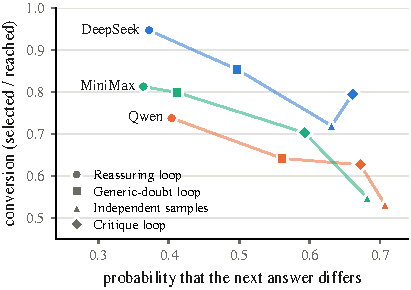
\includegraphics[width=\columnwidth]{figs/conversion.pdf}
  \caption{Conversion against the probability that two consecutive answers differ (for independent samples: that two samples differ). Each line joins the four methods of one model. Methods that make the model change its answer more often select a smaller share of what they reach.}
  \label{fig:conv}
\end{figure}

\paragraph{Selected questions.}
Figure~\ref{fig:forest} shows the differences of Table~\ref{tab:pairs}.

\begin{figure}[t]
  \centering
  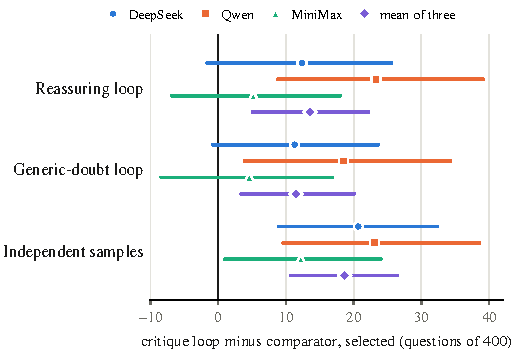
\includegraphics[width=\columnwidth]{figs/forest.pdf}
  \caption{Difference in selected questions between the critique loop and each other method, with 95\% bootstrap intervals.}
  \label{fig:forest}
\end{figure}

\paragraph{Second candidates.}
When the first candidate is wrong and a second one follows, the second is correct in 48 of 204 cases under critique and 26 of 171 under generic doubt on \ds, 61 of 256 and 42 of 220 on \qw, and 35 of 219 and 26 of 168 on \mm.
Under exact matching the critique loop and nine samples reach 122 and 120 questions on \ds, 117 and 93 on \qw, and 98 and 111 on \mm{} (Table~\ref{tab:robust}).

\paragraph{Reach without multiple-choice questions.}
The advantage in reach is not a matter of reaching the key of a multiple-choice question by elimination.
On the 314 questions whose reference answer is not a single letter (this leaves out the multiple-choice questions and two questions with a one-letter answer) the critique loop still reaches more than the generic-doubt loop on every model (34/9, 33/13 and 28/13; $p\le 0.03$).

\paragraph{Reach by subject area.}
This breakdown is descriptive.
Summed over the three models, the questions reached only by the critique loop and only by the reassuring loop are: mathematics (175 questions) 73 and 12; computer science and AI (44) 12 and 2; biology and medicine (41) 29 and 3; physics (40) 14 and 3; humanities and social science (36) 12 and 3; other (31) 9 and 4; chemistry (20) 9 and 0; engineering (13) 1 and 1.
Against the generic-doubt loop the counts are 55 and 20; 12 and 2; 20 and 2; 11 and 3; 9 and 3; 8 and 7; 7 and 1; 3 and 3.
Against the reassuring loop the critique loop reaches more in 8, 7 and 5 of the eight areas on \ds, \qw{} and \mm. Against the generic-doubt loop in 8, 6 and 6.
No area shows the opposite direction when the models are summed.

\paragraph{Choice of benchmark, earlier runs, and how the questions were drawn.}
We list here everything that was run before the study, so that the reader can judge whether the benchmark or the questions were chosen in the light of results.
\emph{Other benchmarks.}
Before this study we measured first answers of deepseek-v4-flash on about 50 questions from each of six benchmarks: AIME 47 of 50 correct, GPQA-Diamond 41 of 50, BBH 40 of 44, MMLU-Pro 43 of 50, MATH-500 45 of 50 and BFCL 45 of 50, which is 89\% overall.
We also ran loops on these benchmarks with deepseek-v4-flash, and tried early versions of the same-model judges there.
An early critic loop, with a different critic and no placebo, ended with 81\% of last answers correct against 76\% to 78\% of first answers on 148 further GPQA-Diamond questions (two runs), and with 90\% against 85\% on 144 questions from AIME, GPQA-Diamond and BBH.
The reassuring loop, run later under changed settings, ended with 86\% against 84\% on the same 148 questions, 94\% against 96\% on the same 144, and 97\% against 97\% on 200 questions from four other task sets, among them MATH-500, MMLU-Pro and BFCL.
Early critic runs on two other models and development runs on at most 50 questions also exist. The summaries of all these runs are kept with the released material.
The two sets of runs differ in reasoning budget and scoring (their first-answer accuracies differ for that reason), neither was scored for reached or selected questions, and the generic-doubt loop and the critique loop of this paper were never run on these benchmarks.
We draw no conclusion from them.
With first answers this often correct, a round of revision pays only if it fixes incorrect answers at several times the rate at which it breaks correct ones (eight times at 89\%; see the break-even point below), and few incorrect answers remain to be fixed.
We therefore turned to a benchmark on which first answers are mostly wrong.
The 33 incorrect first answers were used to build the list of error types of the restricted critic (Appendix~\ref{app:bank}). They support no result in this paper.
\emph{The 400 questions.}
They were drawn in three steps by one rule (text-only questions, stratified by subject, fixed seed): 50, then 150, then 200.
Early versions of the loop were run on the first 200 while the protocol was being developed; nothing was run on the last 200 before the run protocol was frozen (the scoring protocol of Appendix~\ref{app:scoring} was completed afterwards, on all 400).
No question was removed at any step, and every number in this paper comes from runs on all 400 under the frozen protocol.
The results do not depend on the questions seen during development.
On the last 200 questions alone the critique loop reaches more than the reassuring loop on every model (discordant pairs 27/2, 35/5 and 20/3; on the first 200: 25/5, 34/5 and 18/8) and more than the generic-doubt loop (18/6, 19/7 and 17/8; on the first 200: 21/6, 30/9 and 20/5).
Its difference from the reassuring loop in selected questions is $+7.2$, $+11.2$ and $+6.6$ on the last 200 and $+5.2$, $+12.0$ and $-1.3$ on the first 200.
\emph{Methods, models and analyses.}
The generic-doubt loop and the critique loop were specified, with their criteria, after the first runs on the 400 questions and before their own runs; Appendix~\ref{app:prereg} lists what was fixed in advance for each model, and the replacement of the third model before any of its answers was scored.
Every method and model that was run on the 400 questions under the frozen protocol is reported in this paper.

\paragraph{Conversion.}
If critique helped the model pick out a correct answer, the critique loop might select a larger share of what it reaches.
It selects a smaller share: conversion is below that of the reassuring loop by 0.15 on \ds{} (interval \ci{-0.21}{-0.09}), 0.11 on \qw{} (\ci{-0.20}{-0.03}) and 0.11 on \mm{} (\ci{-0.20}{-0.03}).
Part of this is composition: the questions that only the critique loop reaches are ones on which the first answer was wrong, and such questions are harder to select in any method.

\paragraph{Where the selected questions come from.}
Table~\ref{tab:split} splits the questions by which loop reaches them.
The questions that only the critique loop reaches (52, 69 and 38) are the source of its gain: it selects about half of them (27.8, 31.8 and 16.3).
On the questions that both loops reach, the critique loop selects fewer than the reassuring loop on every model ($-10.4$, $-2.5$ and $-4.8$).
The loss is significant on \ds{} and in the pooled data (mean per model $-5.9$, \ci{-10.9}{-1.1}, $p=0.025$).
The net difference in Table~\ref{tab:pairs} is the first effect minus the second and minus the few questions that only the reassuring loop reaches.

This split groups questions by an outcome, so it describes where the gain arises and does not show that critique harms selection: the questions a reassuring loop reaches are mostly those the first answer already had right, which are easy to keep.
Against the generic-doubt loop, on questions both reach, the critique loop is neither better nor worse (mean per model $-0.9$, \ci{-6.6}{4.6}).
The pattern is consistent with doubt of either kind making correct answers somewhat less secure, but our design does not test this directly.

\begin{table}[t]
\centering
\small
\setlength{\tabcolsep}{3.6pt}
\begin{tabular}{@{}l rrr@{}}
\toprule
 & \ds & \qw & \mm \\
\midrule
\multicolumn{4}{@{}l}{\emph{Reached by both loops}} \\
\quad questions & 146 & 113 & 114 \\
\quad selected, critique & 129.6 & 82.3 & 90.6 \\
\quad selected, reassuring & 140.0 & 84.8 & 95.3 \\
\quad difference & $-10.4^{**}$ & $-2.5$ & $-4.8$ \\
\multicolumn{4}{@{}l}{\emph{Reached only by the critique loop}} \\
\quad questions & 52 & 69 & 38 \\
\quad selected, critique & 27.8 & 31.8 & 16.3 \\
\multicolumn{4}{@{}l}{\emph{Reached only by the reassuring loop}} \\
\quad questions & 7 & 10 & 11 \\
\quad selected, reassuring & 5.0 & 6.0 & 6.3 \\
\midrule
Net difference & $+12.4$ & $+23.3$ & $+5.2$ \\
\bottomrule
\end{tabular}
\caption{Where the critique loop's selected questions come from: a descriptive split by an outcome, not a causal decomposition. Its gain over the reassuring loop arises on questions that only it reaches; on questions both reach it selects fewer ($^{**}p<0.01$, permutation test).}
\label{tab:split}
\end{table}

\paragraph{An arithmetic split of the gain in selected questions.}
Write $R$ for reached, $S$ for selected and $C=S/R$ for conversion, with subscripts $c$ for the critique loop and $p$ for the reassuring loop.
Then $S_c-S_p=(R_c-R_p)\,C_p+R_c\,(C_c-C_p)$: what the additional reach would add at the reassuring loop's conversion, plus the effect of the critique loop's different conversion.
The first term is $+42.6$, $+43.6$ and $+22.0$ questions on \ds, \qw{} and \mm. The second is $-30.2$, $-20.3$ and $-16.7$; their sums are the differences of Table~\ref{tab:pairs}, $+12.4$, $+23.3$ and $+5.2$.
The lower conversion thus removes 71\%, 47\% and 76\% of the first term.
This is an identity, not a causal decomposition: the two loops reach different questions.
It shows that the small gain on \mm{} goes with a reach gain half as large as on the other models, and that a loss in conversion is common to all three.
Differences between models in the gain in selected questions: \qw{} minus \ds{} $+10.8$ \ci{-8.8}{31.6}; \qw{} minus \mm{} $+18.0$ \ci{-0.2}{36.8} ($p=0.07$); \ds{} minus \mm{} $+7.2$ \ci{-11.2}{25.1}.
All of this is exploratory.

\paragraph{Selected questions under exact matching.}
When only exact matches count as correct, the first answer is correct on 63, 38 and 51 questions, and the selected counts for the reassuring loop, generic-doubt loop, critique loop and nine samples are 84.0, 82.4, 96.5, 84.6 on \ds; 56.0, 59.0, 68.1, 50.2 on \qw; and 65.2, 66.1, 66.6, 62.9 on \mm.
Critique loop minus reassuring loop: $+12.5$ \ci{0.8}{24.3}, $+12.1$ \ci{-0.7}{24.8}, $+1.4$ \ci{-8.6}{11.8}; mean per model $+8.7$ \ci{1.9}{15.8}.
Critique loop minus nine samples: $+12.0$ \ci{2.1}{22.0}, $+17.9$ \ci{4.6}{30.6}, $+3.6$ \ci{-5.2}{13.5}; mean per model $+11.2$ \ci{4.6}{18.2}.

\paragraph{The first revision.}
Questions repaired and damaged by the first round of feedback: \ds{} reassuring 17 and 7, generic doubt 22 and 13, critique 45 and 20; \qw{} 30 and 13, 40 and 18, 47 and 29; \mm{} 21 and 13, 26 and 12, 27 and 29.

\paragraph{Does the critic hand over answers?}
A critic could help by solving the question and passing its solution on.
If so, its text should contain the solver's next answer, mainly when the change is for the better.
Among changes with a numeric or free-text answer, the critic's text contains the next answer in 2 of 132 changes for the better and 2 of 100 for the worse on \ds, 17 of 159 and 16 of 132 on \qw, and 13 of 115 and 16 of 98 on \mm.
So on \qw{} and \mm{} between 10\% and 16\% of critiques contain the next answer, with no excess among changes for the better.

\paragraph{Sampling at equal cost and the model as selector (\ds).}
With eleven samples, the token cost of the critique loop, the vote selects 138.2 and reaches 193.
When the solver model is given the eleven answers and asked to pick the consensus, with the prompt of \citet{chen2023usc}, it selects 145 ($+6.8$ over the vote, \ci{-1.3}{15.4}).
The critique loop's most frequent answer exceeds this by 12.4 (\ci{-0.7}{25.6}, $p=0.06$).
Applied to the critique loop's own answers, the same selector gives 153, below the most frequent answer (157.4).

\paragraph{When does the loop beat the vote?}
Other studies find a majority vote over samples ahead of sequential revision \citep{wang2025rethinking,mirzaei2026sample}.
We examined three possible reasons in our data. All of this is exploratory.
\emph{Read-out.} Those studies take the last revision. The critique loop's last answer exceeds the most frequent answer of nine samples by 11.3 on \ds{} (\ci{-2.1}{24.2}), 21.0 on \qw{} (\ci{6.7}{36.5}) and 4.3 on \mm{} (\ci{-9.2}{17.4}). Its most frequent answer exceeds it by 20.7, 23.1 and 12.2.
Replaying their protocol more closely, the answer after three rounds of critique against a vote over five samples, gives $+14.2$ (\ci{-0.2}{28.6}), $+3.7$ (\ci{-9.6}{18.0}) and $+6.3$ (\ci{-8.1}{21.1}).
\emph{Answer format.} On the 86 questions whose reference is a single letter, the critique loop's most frequent answer exceeds nine samples by 0.0, 6.2 and 4.4 (no interval excludes zero), and its last answer differs from them by $-5.5$, $+8.7$ and $-1.8$. On the other 314 questions the most frequent answer is ahead by 20.7 (\ci{10.6}{31.4}), 16.9 (\ci{5.6}{29.1}) and 7.8 (\ci{-2.8}{18.5}).
\emph{Difficulty.} We graded each question for a model by how many of the other two models answer it correctly at first (none, one, both). The loop's advantage per question does not grow with difficulty: pooled over models it is 0.03, 0.08 and 0.09 questions per question in the three strata, from hardest to easiest.
So the loop's advantage over the vote is tied to reading the loop by its most frequent answer and to open-form answers, and not to the difficulty of our questions.

\paragraph{A bound on vote splitting.}
Independent samples may write one answer in several ways and so split their vote.
To bound the effect we merge, before voting, all answers to a question that were scored correct. This uses the reference and overstates the effect.
Under the bound the critique loop exceeds nine samples by 13.0 on \ds{} (\ci{2.1}{23.8}), 12.2 on \qw{} (\ci{-2.8}{27.3}) and 5.4 on \mm{} (\ci{-6.2}{17.3}).

\paragraph{The break-even point for revision.}
One round of revision fixes some incorrect answers and breaks some correct ones.
It raises accuracy only if the share of incorrect answers fixed, divided by the share of correct answers broken, exceeds $a/(1-a)$, where $a$ is the accuracy before revision \citep{yang2024confidence}.
With first-answer accuracy of 0.28, 0.17 and 0.20 the bar is 0.39, 0.21 and 0.25. At an accuracy of 0.8 it is 4.
This is one reason why results on hard and easy tasks differ.

\section{Token-Matched and Content Controls}
\label{app:controls}

These controls were run on \qw{} after the main study, on the same 400 questions and from the same first answers.
Each was written down with its tests and with what each outcome would be taken to mean before it was run.
The token-matched control matches total tokens, not the critic call.
The content controls vary whether the feedback is about the question and whether the critic has access to the answer. They are reported as pairwise contrasts, not as a single causal ladder (Table~\ref{tab:controlprops}).
A critic call can act on the solver only through the text it passes on: if the call were made and its output replaced by generic doubts, the solver's input would be that of the generic-doubt loop. We therefore ran no control for the call as such.

\paragraph{Conditions.}
\emph{Token-matched generic doubt}: the generic-doubt loop with one change, its stopping rule. It does not stop on repeated answers. On each question it runs until the solver has spent what the critique loop spent on that question (solver tokens plus one critic call per round of feedback, each call costed at the mean of the replayed calls, 4.8 thousand tokens), with a cap of 100 rounds of feedback.
The round that crosses the budget is kept.
\emph{Mismatched critique}: the critique loop with one change. In round $r$ the solver receives the critique that the critic wrote in round $r$ of the main run for another question, a donor of the same answer type and another subject area whose critiques are of similar length. The critiques are reused in rotation if the donor has fewer rounds. No critic is called.
\emph{Question-only critique}: the critique loop with one change. The critic is shown the question and the labels of the doubts it raised in earlier rounds, which it is asked not to repeat, and neither the solver's answer nor its reasoning. One sentence of its instruction differs from that of the critique loop's critic.

\begin{table}[h]
\centering
\small
\setlength{\tabcolsep}{2.6pt}
\begin{tabular}{@{}l ccccc@{}}
\toprule
 & Critic & About the & Reads the & Written & Tokens \\
 & call & question & answer & each round & \\
\midrule
Generic doubt & no & no & no & no & 21 \\
Token-matched & no & no & no & no & 38 \\
Mismatched & reused & no & no & yes & 15$+$8 \\
Question-only & yes & yes & no & yes & 23$+$9 \\
Critique & yes & yes & yes & yes & 24$+$13 \\
\bottomrule
\end{tabular}
\caption{What differs between the conditions on \qw. \emph{Tokens}: millions, solver plus critic; for the mismatched critique the second figure is what the reused critiques cost when they were first produced. Figures are rounded separately; the critique loop's total is 36.2.}
\label{tab:controlprops}
\end{table}

\paragraph{Runs and checks of the manipulation.}
Every condition completed all 400 questions with no failed call and no answer cut off at the token limit.
The token-matched control spent 38.0 million tokens, 105\% of the critique loop's 36.2 million, and no question reached the cap. It ran 16.7 rounds of feedback per question against 5.4 for the generic-doubt loop and produced 4.5 candidates against 2.9.
Our criterion for matched tokens (95\% to 120\% of the critique loop's total, at most 20 questions at the cap) is met.
The mismatched critiques have the length of the critiques proper (1{,}645 against 1{,}647 characters) and overlap with the words of the question as little as the generic doubts do (Jaccard overlap 0.011 against 0.013; 0.078 for critiques about the question).
The question-only critiques are 90\% as long as the critiques proper, contain three doubts in 99\% of rounds (95\% for the critique loop) and overlap with the question as much (0.078). No two consecutive critiques were identical.
The solver's answer changes after 40\% of rounds under mismatched critique, as under reassurance (40\%), against 56\% under generic doubt, 59\% under question-only critique and 67\% under critique.
The text of a question-only critique contains the solver's next answer in 79 of 1{,}096 changes to a numeric or free-text answer (7\%).

\paragraph{Tests fixed in advance.}
Three primary tests on reach, corrected together by Holm's method (Table~\ref{tab:controltests}).
(i) Critique loop against the token-matched control: 182 against 181 questions, discordant pairs 32/31, $p=1$. Counting only the rounds within the budget, the control reaches 174 (35/27, $p=0.37$).
The token-matched control reaches more than the ordinary generic-doubt loop (42/10, $p<0.001$).
By the reading fixed in advance this is ``consistent with computation''. We do not read it as showing that the content of the feedback is irrelevant.
(ii) Critique loop against the mismatched critique: 72/10, $p<0.001$. The mismatched critique also reaches fewer questions than the generic-doubt loop (9/38, $p<0.001$), which by the reading fixed in advance means that a mismatched critique is harmful and that test (ii) cannot by itself be attributed to a benefit of feedback about the question.
A comparison that was not fixed in advance qualifies this: the mismatched critique reaches as many questions as the reassuring loop (17/20), and the solver changes its answer as rarely, so the solver appears to disregard it more than to be misled by it.
(iii) Critique loop against the question-only critique: 48/27, $p=0.020$, $0.041$ after correction. The question-only critique was not flagged for a difference in length (our criterion: below 70\% of the critique loop's length, or a share of rounds with three doubts that differs by more than 15 points).
Its loop spends 88\% of the critique loop's tokens, and (i) shows that tokens alone raise reach, so the difference cannot be assigned wholly to reading the answer.
It does not reach significantly more than the generic-doubt loop (34/22, $p=0.14$).

\begin{table}[h]
\centering
\small
\setlength{\tabcolsep}{3pt}
\begin{tabular}{@{}l c l@{}}
\toprule
Critique loop against & Reached & Selected \\
\midrule
Token-matched generic doubt & 32/31 & $+22.1$ \ci{9.0}{35.8} \\
Mismatched critique & 72/10$^{***}$ & $+20.6$ \ci{6.5}{36.2} \\
Question-only critique & 48/27$^{*}$ & $+18.7$ \ci{4.9}{32.8} \\
Generic doubt & 49/16$^{***}$ & $+18.5$ \ci{3.9}{34.3} \\
\bottomrule
\end{tabular}
\caption{The critique loop against each control on \qw. \emph{Reached}: questions reached only by the critique loop / only by the control (exact McNemar test; $^{*}p<0.05$ and $^{***}p<0.001$, for the first three rows after Holm's correction). \emph{Selected}: difference with 95\% bootstrap interval; descriptive.}
\label{tab:controltests}
\end{table}

\paragraph{Selected questions.}
Comparisons of selected questions were specified as descriptive.
The controls select 93.5 (mismatched critique), 95.6 (generic doubt), 95.3 (question-only critique) and 92.0 (token-matched) questions, and the reassuring loop 90.8. No two of these differ significantly.
The token-matched control against the ordinary generic-doubt loop: $-3.6$ \ci{-14.2}{7.5}.
The critique loop selects 114.1 (Table~\ref{tab:controltests}).
When only exact matches count as correct, the six loops select 56.0 (reassuring), 55.5 (mismatched critique), 59.0 (generic doubt), 57.4 (question-only critique), 57.4 (token-matched) and 68.1 (critique).
The critique loop is then ahead of the token-matched control by 10.7 \ci{-0.8}{21.8}, of the mismatched critique by 12.6 \ci{1.8}{23.1}, of the question-only critique by 10.7 \ci{-0.5}{22.3}, of the generic-doubt loop by 9.1 \ci{-3.8}{21.8} and of the reassuring loop by 12.1 \ci{-0.7}{24.8}.
Exact matching leaves out correct answers that are written differently from the reference, so it lowers every count. It is a check on the grader, not a better measure.
The share of selected questions that are exact matches is similar in the six loops (0.59 to 0.62), so the smaller margins reflect fewer countable answers and give no sign that the grader favours the critique loop.
Reach under exact matching: 117 for the critique loop against 113 for the token-matched control (discordant pairs 26/22), 76 for the mismatched critique (46/5) and 102 for the question-only critique (32/17).

\paragraph{Continuation to equal tokens.}
The reassuring, mismatched-critique and question-only loops were later continued from their existing runs, without the rule that stops on repeated answers, until each question had spent the tokens of the critique loop on it (for the question-only loop, solver and critic); questions already over that budget were left as they were and are read up to the round that crosses it.
The plan, fixed before the continuation, had three tests on reached questions, critique loop against each continued loop, with Holm correction.
Tokens after alignment: 104\%, 105\% and 109\% of the critique loop's; seven questions of the reassuring loop stopped at the cap of 100 rounds short of the budget (criterion: at most 20).
Critique against question-only: 35/32, $p=0.81$.
Against mismatched: 37/21, $p=0.048$, after correction $0.096$.
Against reassuring: 45/22, $p=0.007$, after correction $0.020$.
Selected questions (descriptive), critique loop minus each loop at equal tokens: $+26.4$ (\ci{12.7}{41.8}) reassuring, $+17.3$ (\ci{3.9}{31.5}) mismatched, $+22.1$ (\ci{9.0}{35.8}) generic doubt, $+22.3$ (\ci{8.4}{36.8}) question-only. With exact matching alone $+11.9$ (\ci{0.2}{23.6}), $+8.1$ (\ci{-1.5}{17.8}), $+10.7$ (\ci{-0.8}{21.8}) and $+9.1$ (\ci{-1.8}{19.8}).
Exact matches make up 60\% to 64\% of the selected questions of each of the five loops.

\paragraph{Token-matched generic doubt on \mm.}
The same control was run on \mm{} with budgets from its critique loop: 42.8 million tokens against 40.4 million (ratio 1.06), no question at the cap.
It reaches 156 questions and selects 96.0.
Critique against token-matched, reached: 21/25, $p=0.66$ (25/22 when only rounds within the budget count).
Token-matched against generic doubt, reached: 39/11, $p<0.001$.
Selected, critique minus token-matched: $+10.9$ (\ci{-0.5}{22.3}); token-matched minus generic doubt: $-6.3$ (\ci{-17.4}{4.2}).

\paragraph{A check of the question-only critiques.}
Thirty question-only critiques, drawn with a fixed seed and shown without any information about correctness, were labelled by one of the authors and then reviewed by the AI assistant, who had seen those labels. The second look is therefore a review, not an independent annotation. None was generic: each refers to quantities, concepts or steps specific to its question. Five give away or point to an answer, for example by deriving the answer's formula, by arguing that no integer solves the equation, or by eliminating options. Two more come close, one by giving the parts of a solution to an open-ended question and one by narrowing a numeric answer to three values. The labels and the review agree on 28 of 30. A critic that sees only the question can thus solve it, and in about a fifth of its critiques the solution reaches the solver. The string check above, which looks for the solver's next answer, finds 7\% because it cannot detect a derivation or an elimination. The question-only critique therefore removes the critic's access to the answer but not the answer itself.

\paragraph{Changes made after a check of run health.}
Before each full run, 16 questions were run and only run statistics were examined (completion, cut-off answers, rounds, tokens, length of feedback). No correctness was computed.
Two settings were changed at that point.
The cap on rounds of the token-matched control was raised from 30 to 100: answers that have settled cost few tokens per round, and with a cap of 30 about 18\% of questions would have stopped short of their budget.
A failed critic call in the question-only control is handled as in the critique loop (one retry, then a neutral sentence for that round; 4 rounds, against 10 in the critique loop) and not by rerunning the question, as first written.
An analysis that cuts the critique loop off at a placebo loop's token budget was also computed before these controls existed. It shortens the critique loop and cannot say what a placebo loop would do with more tokens, and we replaced it by the token-matched control.

\section{Confirmation on HLE-800}
\label{app:confirm}

\paragraph{Design.}
The 800 questions were drawn from the text-only questions of the benchmark after removing the 400 already used, by the rule of the first study (stratified by subject area, fixed seeds), in two draws of 400 that were to be read together.
No question was replaced or removed.
The model is \qw, chosen after the first study as the only model whose gain in selected questions over the reassuring loop excluded zero there; prompts, limits and stopping rules are those of the first study.
The token-matched generic-doubt loop takes its budget for each question from the critique loop's run on these questions (solver and critic tokens as logged) and runs for at most 100 rounds of feedback.
Scoring follows the frozen protocol of Appendix~\ref{app:scoring}, without the adjudication step.
No correctness was inspected before all runs were complete and scored.

\paragraph{Criteria fixed before the runs.}
(i) Token alignment: the token-matched loop spends between 95\% and 120\% of the critique loop's tokens and at most 40 questions stop at the cap of 100 rounds. Otherwise the tests involving it are not judged.
(ii) Two confirmatory tests on selected questions, critique loop minus token-matched loop and critique loop minus reassuring loop, each by a sign-flip permutation test on questions (10,000 permutations, two-sided, direction as hypothesized) with Holm correction over the two.
(iii) One test of equivalence on reached questions: the 90\% bootstrap interval of the difference between the critique loop and the token-matched loop lies within $\pm 33$ questions. The bound is half of what the difference in reach between the critique loop and the ordinary generic-doubt loop on HLE-400 (33) would amount to on 800.
(iv) Secondary and descriptive quantities, including a breakdown by subject area and answer type.
Power was estimated before the runs from the standard errors on HLE-400: for the difference against the token-matched loop, about 99\% if it were as large as on HLE-400 (22 per 400 questions), 81\% at 15 and 51\% at 11. The observed difference is 11.9 per 400 questions.

\paragraph{Results.}
Token alignment: 69.2 million tokens against 66.2 million (ratio 1.045). No question at the cap.
Selected, critique minus token-matched: $+23.8$ (\ci{5.9}{42.3}), $p=0.008$, after correction $0.008$.
Selected, critique minus reassuring: $+36.8$ (\ci{17.4}{57.3}), $p=0.0003$, after correction $0.0006$.
Reached, critique minus token-matched: $-15$, 90\% interval $-32$ to $+2$; discordant pairs 51/66, $p=0.20$.
The criterion is met by one question: with a bound of 30 in place of 33 the test would have been inconclusive.
The lower limit also depends on the bootstrap sample: an independent computation with 10,000 resamples gives $-33$ to $+3$, and a normal approximation $-32.8$ to $+2.8$.
The two sides of the test are therefore not equally secure. That the critique loop reaches no more questions than the token-matched loop is secure (upper limit $+2$ to $+3$ against a margin of 33). That it does not reach materially fewer is on the margin.
Counting only the rounds of the token-matched loop that fit within the budget: selected $+28.3$ (\ci{10.4}{46.8}); reached $-6$ (90\% interval $-24$ to $+12$).

\paragraph{Secondary.}
Reached: critique against reassuring 133/30, against generic doubt 101/40, token-matched against generic doubt 102/26 (all $p<0.001$).
Selected: critique minus generic doubt $+22.1$ (\ci{4.4}{40.5}); token-matched minus generic doubt $-1.8$ (\ci{-15.8}{13.5}).
Exact matches only: the two confirmatory differences are $+17.3$ (\ci{1.4}{33.0}) and $+25.9$ (\ci{8.2}{42.5}), and the difference in reached questions is $-15$ (90\% interval $-31$ to $+1$); exact matches make up 66\% to 67\% of the selected questions of each of the four loops.
Feedback rounds per question: 3.9, 5.2, 15.2 and 6.3 for the reassuring, generic-doubt, token-matched and critique loops; candidates per question 2.0, 2.7, 4.2 and 3.4.

\paragraph{By subject area and answer type.}
Selected questions, critique loop minus token-matched loop, by subject: Mathematics (364 questions) $+7.7$, Biology and Medicine (82) $+6.2$, Computer Science (82) $+1.2$, Physics (74) $+5.2$, Humanities and Social Science (72) $+0.5$, Other (66) $+1.0$, Chemistry (37) $+1.0$, Engineering (23) $+1.0$: positive in eight of eight.
Against the reassuring loop it is positive in six of eight (Computer Science $-0.8$, Engineering $-1.0$), and against the ordinary generic-doubt loop in six of eight (Humanities $-3.3$, Engineering $-0.5$).
In reached questions the token-matched loop is ahead of the critique loop in Mathematics (32 against 12 discordant questions) and Physics (9 against 3), and behind or level elsewhere.
By answer type the difference in selected questions against the token-matched loop is $+18.4$ on 599 open-form questions and $+5.5$ on 201 multiple-choice questions.
No test was run within a stratum.

\paragraph{Independent re-computation.}
The confirmatory and primary tests of this appendix and of Appendix~\ref{app:controls} were recomputed with SciPy (exact binomial test on discordant pairs; paired permutation test and percentile bootstrap with 10,000 resamples and its own random numbers).
Discordant counts, differences and exact $p$-values are identical; permutation $p$-values differ by at most 0.0012 and interval limits by at most 1.3 questions.
No conclusion changes except that the equivalence interval touches its margin, as noted above.

\paragraph{Not in the plan.}
By draw, the difference in selected questions against the token-matched loop is $+4.8$ (\ci{-6.6}{17.5}) on the first draw of HLE-800 and $+19.0$ (\ci{5.9}{32.0}) on the second. Against the reassuring loop $+13.6$ (\ci{1.0}{27.9}) and $+23.2$ (\ci{8.5}{37.1}).
Pooled with HLE-400 (1,200 in all; exploratory, since HLE-400 gave rise to the hypothesis) the two differences are $+46.0$ (\ci{23.0}{69.2}) and $+60.1$ (\ci{35.0}{85.6}).

\paragraph{Runs added after the read-out.}
The plan above did not include independent samples or the question-only critique on HLE-800.
Both were added after the tests above had been read, with their tests written before they were run: critique loop minus nine independent samples in selected questions, which repeats the test of the first study, and critique loop minus the question-only critique continued to equal tokens, corrected together.
The first holds ($+27.2$, \ci{6.8}{47.2}, corrected $p=0.012$). The second does not ($+11.8$, \ci{-7.4}{29.4}).
Nine samples select 178.1 and reach 329. The question-only critique selects 191.4 at its natural stop and 193.5 at equal tokens.
\ds{} was then run on the same 800 questions with the same tests and criteria, fixed before its runs: critique minus token-matched $-7.2$ (\ci{-23.9}{9.3}) and minus reassuring $-1.9$ (\ci{-18.6}{15.3}), neither confirmed; minus nine samples $+29.6$ (\ci{12.4}{47.8}, corrected $p=0.0024$), confirmed; reach, critique minus token-matched $-1$ (90\% interval $-16$ to $+15$), equivalent within $\pm27$.
On \ds{} the first answer is correct on 198 questions. The reassuring, generic-doubt, token-matched and critique loops select 256.2, 248.5, 261.5 and 254.2 and reach 291, 311, 371 and 370.
The difference between the models in critique minus token-matched is $+31.0$ (\ci{5.9}{55.7}; descriptive).
A repeat of the critique and token-matched loops on the first draw of HLE-800 with \qw{} gave selected counts of 95.8 and 89.2 against 98.5 and 93.6, and differences between them of $+4.8$, $+9.2$, $+2.2$ and $+6.5$ for the four pairings of runs.

\section{Samples at Equal Tokens and USC}
\label{app:e2}

\paragraph{Design.}
For each model and question, the nine existing samples were continued at temperature 0.7 with the same prompt until their tokens (prompt and completion, without the first answer) reached the critique loop's budget on that question, with at most 100 samples. The sample that crosses the budget is kept.
For USC the model was shown all samples of a question and asked which response is most consistent with the others, with the prompt and parsing rules of the first study's USC comparison (Appendix~\ref{app:first}). If the choice could not be parsed after one retry, the most frequent answer was used (3 questions on \qw, 21 on \ds).
New samples were scored by the frozen protocol. The nine existing samples keep their scores.
Token alignment had to be between 95\% and 120\% of the budget with at most 40 questions at the cap. It was 118\% (1 at the cap) on \qw{} and 115\% (10) on \ds.

\paragraph{Results.}
Selected and reached questions: critique loop 205.3 and 348 on \qw, 254.2 and 370 on \ds; samples at equal tokens 180.0 and 385, 229.0 and 397; USC 183.0 and 235.0 selected; nine samples 178.1 and 329, 224.7 and 361.
The tests are in Table~\ref{tab:core}.
Samples at equal tokens against nine samples: selected $+1.9$ (\ci{-7.1}{10.6}) and $+4.4$ (\ci{-3.0}{11.6}); reached 56/0 and 36/0.
USC against the plurality of the same samples: $+3.0$ (\ci{-8.1}{13.5}) and $+6.0$ (\ci{-3.0}{15.0}).
Against the placebo loops, samples at equal tokens select $+11.5$ (\ci{-7.1}{29.3}) and $-27.1$ (\ci{-45.0}{-8.6}) relative to the reassuring loop, and $-1.5$ and $-32.4$ relative to the token-matched loop.
Exact matches only: critique minus samples $+28.6$ (\ci{10.2}{47.5}) and $+17.2$ (\ci{2.8}{31.6}); critique minus USC $+41.3$ (\ci{21.7}{61.5}) and $+23.6$ (\ci{9.0}{38.5}).
By answer type, critique minus samples: open-form (599) $+24.3$ (\ci{7.8}{39.7}) and $+19.8$ (\ci{5.7}{33.6}); multiple choice (201) $+1.0$ (\ci{-11.5}{13.4}) and $+5.4$ (\ci{-3.0}{13.9}).

\paragraph{Tokens.}
Tokens are prompt plus completion tokens as billed, reasoning included. For samples the first answer is not counted, for loops it is.
The number of samples differs widely between questions: a question whose samples are short and whose budget is large receives many samples, one whose first nine samples already exceed the budget receives no more (211 of the 800 BBEH questions).
The mean number of samples therefore cannot be multiplied by a mean cost per sample.
The totals are 78.3 against 66.2 million tokens on \qw, 132.7 against 115.1 on \ds, and 108.9 against 96.4 on BBEH.

\paragraph{Further checks (descriptive).}
These were added after a review of a draft and computed once (Table~\ref{tab:supp}).
\emph{Within the budget}: only the samples whose cumulative tokens stay within the budget are counted (16.7, 15.1 and 19.4 per question).
\emph{Without the first answer}: the loop's list starts at its first revised answer.
\emph{Last answer}: the loop is read by its last answer and the samples by their vote.
\emph{Merged}: in both methods all candidates scored correct are merged into one before the vote. This uses the reference and bounds from above what a vote could gain if every correct answer were written the same way.
The critique loop runs 6.3, 6.0 and 6.9 rounds of feedback per question, each a critic call followed by a solver call. The samples can be drawn in parallel.
On \ds{} 5.4\% of the critique loop's answers and 4.2\% of the samples are cut off at the token limit and count as incorrect. On \qw{} almost none.
On BBEH the critique loop is ahead of the samples in seven of the ten tasks, most on temporal sequence ($+13.2$) and hyperbaton ($+12.0$).

\begin{table}[h]
\centering
\small
\setlength{\tabcolsep}{2.2pt}
\begin{tabular}{@{}l ccc@{}}
\toprule
Critique $-$ samples & \qw & \ds & BBEH \\
\midrule
Selected, as read out & $+25.3$ & $+25.2$ & $+34.0$ \\
\quad within the budget & $+28.5$ & $+26.4$ & $+52.5$ \\
\quad no first answer & $+29.1$ & $+26.5$ & $+39.7$ \\
\quad last answer & $+27.0$ & $+25.0$ & $+0.5$ \\
\quad merged & $+9.3$ & $+19.2$ & $+27.3$ \\
Reached, as read out & $-37$ & $-27$ & $-20$ \\
\quad within the budget & $-17$ & $-8$ & $+3$ \\
\bottomrule
\end{tabular}
\caption{The comparison at equal tokens under other readings. Intervals: last answer on BBEH \ci{-24.5}{25.5}; merged \ci{-13.3}{31.5}, \ci{2.8}{36.5} and \ci{7.2}{49.4}; all other intervals for selected questions exclude zero. Reached within the budget: discordant pairs 63/80, 53/61 and 61/58. Descriptive.}
\label{tab:supp}
\end{table}

\section{The Second Benchmark}
\label{app:bbeh}

\paragraph{Choice of benchmark and tasks.}
Three candidate benchmarks were screened with \qw's first answers only, under a rule fixed before the screening: first-answer accuracy between 10\% and 40\% leaves room for revision, above 80\% does not.
GSM8K \citep{cobbe2021gsm8k} gave 97.5\% (200 questions) and OlymMATH \citep{sun2025olymmath} 97\% on its easy and 72\% on its hard part (100 each, official scorer). Neither was run further.
BBEH gave 48.1\% over 805 questions (35 per task), with tasks ranging from 11\% to 97\%, so the rule was applied per task.
Hard tasks (10\%--40\%): multistep arithmetic, NYCC, geometric shapes, SportQA, hyperbaton, temporal sequence, zebra puzzles, Linguini, sarcasm triples, shuffled objects.
Easy tasks (above 80\%): time arithmetic, object counting, BoardgameQA.
The ten tasks in between were not run.
The questions used in the study (80 per task) were drawn with a fixed seed from those not used in the screening.
Prompts, limits and stopping rules are those of HLE, except for the answer format that BBEH requires.
Answers are scored with the benchmark's own scorer. Two answers are the same candidate if the scorer's normalization makes them equal.

\paragraph{Hard tasks.}
First answer 263 of 800.
Selected and reached: reassuring 379.9 and 465, generic doubt 388.9 and 510, token-matched 371.9 and 576, critique 390.5 and 591, nine samples 344.4 and 547, samples at equal tokens 356.5 and 611, token-matched at temperature 0.7 368.0 and 582.
Tokens (millions): 48.1, 57.4, 100.6, 96.4, 69.7, 108.9 and 100.7.
Fixed tests: critique minus token-matched $+18.6$ (\ci{-3.3}{41.4}), minus reassuring $+10.6$ (\ci{-11.3}{33.5}), minus nine samples $+46.1$ (\ci{25.8}{67.1}, confirmed); reach, critique minus token-matched $+15$ (90\% interval $-2$ to $+34$, inconclusive against $\pm33$).
At equal tokens: Table~\ref{tab:core}; loop at temperature 0.7 minus samples $+11.6$ (\ci{-9.6}{31.6}), not confirmed.
Descriptive: critique minus loop at temperature 0.7 $+22.5$ (\ci{-0.9}{44.4}); loop at temperature 0.7 minus at 0 $-3.9$ (\ci{-22.5}{15.9}); samples at equal tokens minus nine samples $+12.0$ (\ci{-0.4}{24.2}).
The critique loop is ahead of the reassuring loop in selected questions in seven of the ten tasks.

\paragraph{Easy tasks.}
First answer 195 of 240.
Selected: reassuring 222.5, generic doubt 227.5, token-matched 226.5, critique 223.8, nine samples 225.5; critique minus reassuring $+1.3$ (\ci{-5.2}{8.3}).
When first answers are mostly right, no loop changes much.

\paragraph{Registered predictions.}
Before the read-out we registered predictions from a hypothesis developed on the HLE data: that the loop helps mainly on questions where the model is unsure of its first answer, measured by how many of nine samples agree with it.
P1: under critique the most frequent answer stays the first answer more often the more the samples agree, at least 85\% of the time when 7 to 9 agree, with no more than 0.10 between questions whose first answer is right or wrong.
The first two parts held (0.27, 0.74 and 0.92), the third did not (0.97 against 0.86, a gap of 0.108).
P2: at least two thirds of the critique loop's gain over the reassuring loop comes from unsure questions with a wrong first answer. It was 53\%.
P3 (no gain on the easy tasks) and P4 (high agreement goes with correct first answers far more often on the easy tasks) held.
P5 predicted the gain on the hard tasks from per-question effects on HLE ($+20.9$, inside the observed interval) and on the easy tasks ($-6.1$, outside the observed interval).
By the rule registered with them, the failures of P1 and P2 mean the hypothesis is not supported on this benchmark.

\section{Removing the Previous Answer}
\label{app:memory}

\paragraph{Design.}
In the token-matched generic-doubt loop on the hard BBEH tasks, we changed only the solver's message.
In the \emph{no-memory} condition (800 questions) the previous answer is not shown, the first sentence refers to ``your previous attempt (not shown)'', and the sentence permitting the solver to keep its answer is removed. In the \emph{no-permission} condition (400 questions, the first 40 of each task) the previous answer is shown and only that sentence is removed.
Feedback, budgets and all other settings are unchanged, and no conversation history is carried between rounds in any condition.
The check of the manipulation, fixed in advance, required the share of questions whose first-round answer repeats the first answer to differ from the original loop by at least 5 points at $p<0.05$ (in either direction).
The one confirmatory test was selected (original) $-$ selected (no memory) $>0$, judged only if the check passed and tokens were aligned.
A second stage on HLE was to be run only if this test held.

\paragraph{Results.}
Tokens 104\% of the budget, none at the cap.
Check: 0.41 against 0.50 ($p<0.001$), so the solver repeats its first answer less often without seeing it.
Selected 359.5 against 371.9: difference $+12.4$ (\ci{-6.0}{30.9}), $p=0.20$, not confirmed. The second stage was not run.
Descriptive: without memory the loop reaches 592 questions against 576 and converts less (0.61 against 0.65). On the 400 questions, the part attributable to showing the answer is $+6.4$ (\ci{-6.4}{19.3}) and to the permission $+2.0$ (\ci{-10.3}{14.1}).
The direction is the one a role for the previous answer would predict, but the effect, if any, is too small to establish here.

\section{Three Properties of a Model (Exploratory)}
\label{app:props}

This appendix records a direction we explored and did not establish.
If a loop selects well by exploiting what the model already knows about its own answers, three properties of the model should matter, and each can be measured without a reference to the loop's outcome (Table~\ref{tab:props}).

\emph{Signal.} Does the model's agreement with itself indicate whether its first answer is correct?
For each question we count how many of nine independent samples give the first answer, and compute the area under the ROC curve of that count as a score for the correctness of the first answer. A value of 0.5 means no information.
\emph{Use.} When the solver is asked again without any information, does it keep correct answers more often than incorrect ones? This is the ratio of the two keep probabilities under the reassuring loop (Table~\ref{tab:keep}).
\emph{Critic.} Does the critic doubt incorrect answers more than correct ones? This is the ratio of doubts per round (Section~\ref{sec:mech}).

\begin{table}[h]
\centering
\small
\setlength{\tabcolsep}{2.4pt}
\begin{tabular}{@{}l ccc@{}}
\toprule
 & \qw, & \ds, & \qw, \\
 & HLE-800 & HLE-800 & BBEH-800 \\
\midrule
Signal (area under ROC) & .56 & .63 & .75 \\
 & \ci{.51}{.61} & \ci{.59}{.67} & \ci{.71}{.78} \\
First answer correct when & & & \\
\quad 7--9 samples agree with it & 18\% & 38\% & 55\% \\
\quad 0--3 samples agree with it & 16\% & 19\% & 18\% \\
Use (keep correct / incorrect) & 1.07 & 1.18 & 1.89 \\
Critic (doubts, inc.\ / cor.) & 1.00 & 1.02 & 1.00 \\
\midrule
Critique $-$ reassuring, selected & $+36.8$ & $-1.9$ & $+10.6$ \\
\bottomrule
\end{tabular}
\caption{Three properties of a model, measured per setting, and the critique loop's gain in selected questions over the reassuring loop. Exploratory.}
\label{tab:props}
\end{table}

The critic carries no signal in any setting.
The model's own signal is weakest for \qw{} on HLE-800: when seven or more of nine samples agree with the first answer, that answer is correct only 18\% of the time, barely more often than when few agree.
This is also the setting in which the solver hardly distinguishes correct from incorrect answers when merely asked again, and the one in which the critique adds most.
For \ds{} on HLE-800 and for \qw{} on BBEH-800 the signal is stronger, the solver uses it without a critique, and the critique adds little or nothing.
The pattern suggests that a critique helps where a model is confidently wrong, by forcing it off answers it would otherwise repeat.

We do not claim this.
There are three settings, the properties were chosen after seeing the data, and two quantitative predictions derived from the same idea failed on BBEH (Appendix~\ref{app:bbeh}).
We report it because the properties are cheap to measure before a loop is run, and whether they predict when a critique pays is a question a larger set of models could answer.

\section{The Model as Judge}
\label{app:judges}
\label{sec:judges}

Many reached questions remain unselected (41, 68 and 45 in the critique loop).
Could the model recover them by judging its own changes of answer?
We tested this once, on \ds{} and with a variant of the critic that must choose its doubts from a fixed list (Appendix~\ref{app:bank}).
The same model acted as a \emph{judge} of every step from one answer to a different one, in three ways and without a reference answer, and its verdicts adjusted the votes of the candidates.
No judge selected more questions than the unadjusted most frequent answer (Table~\ref{tab:judges}).
Where a judge disagreed with a rule that looks only at the votes, which is the only place it can alter the outcome, the three judges were right 49\%, 45\% and 49\% of the time. With 37 to 150 such disagreements, an accuracy of up to about 65\% cannot be excluded.

\paragraph{Details.}
The judge study uses \ds{} and the restricted critic of Appendix~\ref{app:bank}.
The three judges rate a change of answer in different ways: by rating the new answer. By rating it with the question in view and quoting the step objected to; and by deciding whether the critic's doubt before the change was justified.
Their verdicts adjust the votes of the candidates, with weights fitted on half of the questions and applied to the other half.
The vote-count rule guesses that a change was an improvement if the new answer ends with at least as many votes as the old one.
We call a step from one answer to a different answer in consecutive rounds a \emph{change}.
The loops contain 1{,}199 changes, of which 303 \emph{matter}: 160 turn an incorrect answer into a correct one and 143 do the opposite.
The loop reaches 192 questions.
The second and third judge are better than chance on the changes that matter and received a definite verdict (59\% of 303 and 66\% of 183).
In this analysis ties in the vote are resolved in favour of the more recent answer, as the judges' adjustments require an order. The most frequent answer is then correct on 154 questions (150.9 under random ties).
If every harmful change could be undone, about 173 questions would be selected. If every change that the solver attributes to the feedback were undone, about 149. Both figures were computed before three loops were rerun after interface failures.
Judge 1 gives a definite verdict on 98 of the 303 changes that matter and is right on 56.
A sweep over 81 ways of combining verdicts and votes gains at most two questions in-sample and none when the best rule on one half is applied to the other.

\begin{table}[h]
\centering
\small
\setlength{\tabcolsep}{3.5pt}
\begin{tabular}{@{}l ccc@{}}
\toprule
 & Judge 1 & Judge 2 & Judge 3 \\
\midrule
Accuracy on changes that matter & .57 & .59 & .66 \\
Selected, first half (vote: 76) & 76 & 72 & 71 \\
Selected, second half (vote: 78) & 77 & 75 & 77 \\
Accuracy where judge and & 18/37 & 68/150 & 32/66 \\
\quad vote-count rule disagree & (.49) & (.45) & (.49) \\
\bottomrule
\end{tabular}
\caption{Same-model judges on \ds. A change \emph{matters} if it turns an incorrect answer into a correct one or the reverse. \emph{Selected}: questions selected on one half when the judge's verdicts, weighted on the other half, adjust the vote; the unadjusted vote selects 76 and 78 (ties resolved towards the more recent answer). \emph{Vote-count rule}: a change is an improvement if the new answer ends with at least as many votes as the old one.}
\label{tab:judges}
\end{table}


Judge 1 scores three aspects of the new answer (disconnection from earlier steps, contradiction, a locatable error) and votes against the answer when any score is high. It returned a verdict on 1{,}178 of the 1{,}199 changes.
Judge 2 adds the question and a required quotation of the step objected to.
Judge 3 receives the question, the critic's doubt and the criticized answer and decides whether the doubt was warranted. A verdict requires agreement across two presentations in swapped order.
Judges 2 and 3 cover all changes.
The weights are likelihood ratios added in log space; ratios with intervals that exclude one were obtained for Judge 2 (0.73 and 1.75 for its two verdicts) and Judge 3 (0.51 and 1.84), not for Judge 1.
The 81 combination rules vary where a verdict acts, the weights of the two verdicts, and a restriction to questions with a close vote; their in-sample best results are 154, 156 and 155 against 154 for the vote.
Of the 38 reached and unselected questions, 10 are ties, 11 are lost by one vote and 17 by more.

Why is 66\% accuracy on single changes not enough?
Among the 116 questions that have both a correct and an incorrect candidate, overturning the most frequent answer helps on 38 (33\%).
At that base rate a judge that is right with probability $p$ overturns correctly with probability $0.33p/(0.33p+0.67(1-p))$, which exceeds one half only if $p>0.67$.

\end{document}
